\documentclass[1p]{elsarticle_modified}
%\bibliographystyle{elsarticle-num}

%\usepackage[colorlinks]{hyperref}
%\usepackage{abbrmath_seonhwa} %\Abb, \Ascr, \Acal ,\Abf, \Afrak
\usepackage{amsfonts}
\usepackage{amssymb}
\usepackage{amsmath}
\usepackage{amsthm}
\usepackage{scalefnt}
\usepackage{amsbsy}
\usepackage{kotex}
\usepackage{caption}
\usepackage{subfig}
\usepackage{color}
\usepackage{graphicx}
\usepackage{xcolor} %% white, black, red, green, blue, cyan, magenta, yellow
\usepackage{float}
\usepackage{setspace}
\usepackage{hyperref}

\usepackage{tikz}
\usetikzlibrary{arrows}

\usepackage{multirow}
\usepackage{array} % fixed length table
\usepackage{hhline}

%%%%%%%%%%%%%%%%%%%%%
\makeatletter
\renewcommand*\env@matrix[1][\arraystretch]{%
	\edef\arraystretch{#1}%
	\hskip -\arraycolsep
	\let\@ifnextchar\new@ifnextchar
	\array{*\c@MaxMatrixCols c}}
\makeatother %https://tex.stackexchange.com/questions/14071/how-can-i-increase-the-line-spacing-in-a-matrix
%%%%%%%%%%%%%%%

\usepackage[normalem]{ulem}

\newcommand{\msout}[1]{\ifmmode\text{\sout{\ensuremath{#1}}}\else\sout{#1}\fi}
%SOURCE: \msout is \stkout macro in https://tex.stackexchange.com/questions/20609/strikeout-in-math-mode

\newcommand{\cancel}[1]{
	\ifmmode
	{\color{red}\msout{#1}}
	\else
	{\color{red}\sout{#1}}
	\fi
}

\newcommand{\add}[1]{
	{\color{blue}\uwave{#1}}
}

\newcommand{\replace}[2]{
	\ifmmode
	{\color{red}\msout{#1}}{\color{blue}\uwave{#2}}
	\else
	{\color{red}\sout{#1}}{\color{blue}\uwave{#2}}
	\fi
}

\newcommand{\Sol}{\mathcal{S}} %segment
\newcommand{\D}{D} %diagram
\newcommand{\A}{\mathcal{A}} %arc


%%%%%%%%%%%%%%%%%%%%%%%%%%%%%5 test

\def\sl{\operatorname{\textup{SL}}(2,\Cbb)}
\def\psl{\operatorname{\textup{PSL}}(2,\Cbb)}
\def\quan{\mkern 1mu \triangleright \mkern 1mu}

\theoremstyle{definition}
\newtheorem{thm}{Theorem}[section]
\newtheorem{prop}[thm]{Proposition}
\newtheorem{lem}[thm]{Lemma}
\newtheorem{ques}[thm]{Question}
\newtheorem{cor}[thm]{Corollary}
\newtheorem{defn}[thm]{Definition}
\newtheorem{exam}[thm]{Example}
\newtheorem{rmk}[thm]{Remark}
\newtheorem{alg}[thm]{Algorithm}

\newcommand{\I}{\sqrt{-1}}
\begin{document}

%\begin{frontmatter}
%
%\title{Boundary parabolic representations of knots up to 8 crossings}
%
%%% Group authors per affiliation:
%\author{Yunhi Cho} 
%\address{Department of Mathematics, University of Seoul, Seoul, Korea}
%\ead{yhcho@uos.ac.kr}
%
%
%\author{Seonhwa Kim} %\fnref{s_kim}}
%\address{Center for Geometry and Physics, Institute for Basic Science, Pohang, 37673, Korea}
%\ead{ryeona17@ibs.re.kr}
%
%\author{Hyuk Kim}
%\address{Department of Mathematical Sciences, Seoul National University, Seoul 08826, Korea}
%\ead{hyukkim@snu.ac.kr}
%
%\author{Seokbeom Yoon}
%\address{Department of Mathematical Sciences, Seoul National University, Seoul, 08826,  Korea}
%\ead{sbyoon15@snu.ac.kr}
%
%\begin{abstract}
%We find all boundary parabolic representation of knots up to 8 crossings.
%
%\end{abstract}
%\begin{keyword}
%    \MSC[2010] 57M25 
%\end{keyword}
%
%\end{frontmatter}

%\linenumbers
%\tableofcontents
%
\newcommand\colored[1]{\textcolor{white}{\rule[-0.35ex]{0.8em}{1.4ex}}\kern-0.8em\color{red} #1}%
%\newcommand\colored[1]{\textcolor{white}{ #1}\kern-2.17ex	\textcolor{white}{ #1}\kern-1.81ex	\textcolor{white}{ #1}\kern-2.15ex\color{red}#1	}

{\Large $\underline{12a_{0154}~(K12a_{0154})}$}

\setlength{\tabcolsep}{10pt}
\renewcommand{\arraystretch}{1.6}
\vspace{1cm}\begin{tabular}{m{100pt}>{\centering\arraybackslash}m{274pt}}
\multirow{5}{120pt}{
	\centering
	\includegraphics[width=112pt]{../../../GIT/diagram.site/Diagrams/png/955_12a_0154.png}\\
\ \ \ A knot diagram\footnotemark}&
\allowdisplaybreaks
\textbf{Linearized knot diagam} \\
\cline{2-2}
 &
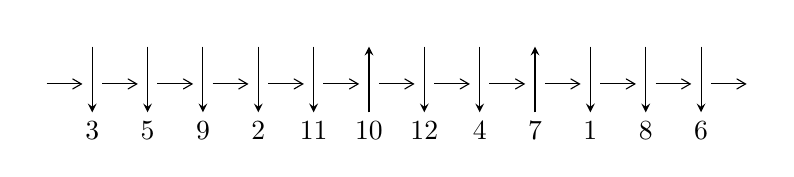
\begin{tikzpicture}[x=20pt, y=17pt]
	% nodes
	\node (C0) at (0, 0) {};
	\node (C1) at (1, 0) {};
	\node (C1U) at (1, +1) {};
	\node (C1D) at (1, -1) {3};

	\node (C2) at (2, 0) {};
	\node (C2U) at (2, +1) {};
	\node (C2D) at (2, -1) {5};

	\node (C3) at (3, 0) {};
	\node (C3U) at (3, +1) {};
	\node (C3D) at (3, -1) {9};

	\node (C4) at (4, 0) {};
	\node (C4U) at (4, +1) {};
	\node (C4D) at (4, -1) {2};

	\node (C5) at (5, 0) {};
	\node (C5U) at (5, +1) {};
	\node (C5D) at (5, -1) {11};

	\node (C6) at (6, 0) {};
	\node (C6U) at (6, +1) {};
	\node (C6D) at (6, -1) {10};

	\node (C7) at (7, 0) {};
	\node (C7U) at (7, +1) {};
	\node (C7D) at (7, -1) {12};

	\node (C8) at (8, 0) {};
	\node (C8U) at (8, +1) {};
	\node (C8D) at (8, -1) {4};

	\node (C9) at (9, 0) {};
	\node (C9U) at (9, +1) {};
	\node (C9D) at (9, -1) {7};

	\node (C10) at (10, 0) {};
	\node (C10U) at (10, +1) {};
	\node (C10D) at (10, -1) {1};

	\node (C11) at (11, 0) {};
	\node (C11U) at (11, +1) {};
	\node (C11D) at (11, -1) {8};

	\node (C12) at (12, 0) {};
	\node (C12U) at (12, +1) {};
	\node (C12D) at (12, -1) {6};
	\node (C13) at (13, 0) {};

	% arrows
	\draw[->,>={angle 60}]
	(C0) edge (C1) (C1) edge (C2) (C2) edge (C3) (C3) edge (C4) (C4) edge (C5) (C5) edge (C6) (C6) edge (C7) (C7) edge (C8) (C8) edge (C9) (C9) edge (C10) (C10) edge (C11) (C11) edge (C12) (C12) edge (C13) ;	\draw[->,>=stealth]
	(C1U) edge (C1D) (C2U) edge (C2D) (C3U) edge (C3D) (C4U) edge (C4D) (C5U) edge (C5D) (C6D) edge (C6U) (C7U) edge (C7D) (C8U) edge (C8D) (C9D) edge (C9U) (C10U) edge (C10D) (C11U) edge (C11D) (C12U) edge (C12D) ;
	\end{tikzpicture} \\
\hhline{~~} \\& 
\textbf{Solving Sequence} \\ \cline{2-2} 
 &
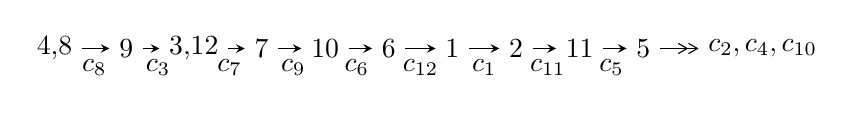
\begin{tikzpicture}[x=23pt, y=7pt]
	% node
	\node (A0) at (-1/8, 0) {4,8};
	\node (A1) at (1, 0) {9};
	\node (A2) at (33/16, 0) {3,12};
	\node (A3) at (25/8, 0) {7};
	\node (A4) at (33/8, 0) {10};
	\node (A5) at (41/8, 0) {6};
	\node (A6) at (49/8, 0) {1};
	\node (A7) at (57/8, 0) {2};
	\node (A8) at (65/8, 0) {11};
	\node (A9) at (73/8, 0) {5};
	\node (C1) at (1/2, -1) {$c_{8}$};
	\node (C2) at (3/2, -1) {$c_{3}$};
	\node (C3) at (21/8, -1) {$c_{7}$};
	\node (C4) at (29/8, -1) {$c_{9}$};
	\node (C5) at (37/8, -1) {$c_{6}$};
	\node (C6) at (45/8, -1) {$c_{12}$};
	\node (C7) at (53/8, -1) {$c_{1}$};
	\node (C8) at (61/8, -1) {$c_{11}$};
	\node (C9) at (69/8, -1) {$c_{5}$};
	\node (A10) at (11, 0) {$c_{2},c_{4},c_{10}$};

	% edge
	\draw[->,>=stealth]	
	(A0) edge (A1) (A1) edge (A2) (A2) edge (A3) (A3) edge (A4) (A4) edge (A5) (A5) edge (A6) (A6) edge (A7) (A7) edge (A8) (A8) edge (A9) ;
	\draw[->>,>={angle 60}]	
	(A9) edge (A10);
\end{tikzpicture} \\ 

\end{tabular} \\

\footnotetext{
The image of knot diagram is generated by the software ``\textbf{Draw programme}" developed by Andrew Bartholomew(\url{http://www.layer8.co.uk/maths/draw/index.htm\#Running-draw}), where we modified some parts for our purpose(\url{https://github.com/CATsTAILs/LinksPainter}).
}\phantom \\ \newline 
\centering \textbf{Ideals for irreducible components\footnotemark of $X_{\text{par}}$} 
 
\begin{align*}
I^u_{1}&=\langle 
1.02998\times10^{761} u^{152}+2.57836\times10^{761} u^{151}+\cdots+1.06742\times10^{765} b+1.14062\times10^{766},\\
\phantom{I^u_{1}}&\phantom{= \langle  }-2.20954\times10^{765} u^{152}+1.24228\times10^{765} u^{151}+\cdots+2.61518\times10^{768} a-1.91271\times10^{769},\\
\phantom{I^u_{1}}&\phantom{= \langle  }u^{153}- u^{152}+\cdots-100352 u+25088\rangle \\
I^u_{2}&=\langle 
-17789137958 u^{23}+33220776343 u^{22}+\cdots+123456179965 b+41044745272,\\
\phantom{I^u_{2}}&\phantom{= \langle  }622863190774 u^{23}-45963389324 u^{22}+\cdots+123456179965 a+2100783655234,\\
\phantom{I^u_{2}}&\phantom{= \langle  }u^{24}+6 u^{22}+\cdots+3 u+1\rangle \\
\\
I^v_{1}&=\langle 
a,\;-82026 v^8-2033115 v^7+\cdots+764761 b+1552510,\\
\phantom{I^v_{1}}&\phantom{= \langle  }7 v^9+3 v^8+2 v^7-14 v^6-23 v^5+33 v^4- v^3-8 v^2+v+1\rangle \\
\end{align*}
\raggedright * 3 irreducible components of $\dim_{\mathbb{C}}=0$, with total 186 representations.\\
\footnotetext{All coefficients of polynomials are rational numbers. But the coefficients are sometimes approximated in decimal forms when there is not enough margin.}
\newpage
\renewcommand{\arraystretch}{1}
\centering \section*{I. $I^u_{1}= \langle 1.03\times10^{761} u^{152}+2.58\times10^{761} u^{151}+\cdots+1.07\times10^{765} b+1.14\times10^{766},\;-2.21\times10^{765} u^{152}+1.24\times10^{765} u^{151}+\cdots+2.62\times10^{768} a-1.91\times10^{769},\;u^{153}- u^{152}+\cdots-100352 u+25088 \rangle$}
\flushleft \textbf{(i) Arc colorings}\\
\begin{tabular}{m{7pt} m{180pt} m{7pt} m{180pt} }
\flushright $a_{4}=$&$\begin{pmatrix}0\\u\end{pmatrix}$ \\
\flushright $a_{8}=$&$\begin{pmatrix}1\\0\end{pmatrix}$ \\
\flushright $a_{9}=$&$\begin{pmatrix}1\\u^2\end{pmatrix}$ \\
\flushright $a_{3}=$&$\begin{pmatrix}u\\u^3+u\end{pmatrix}$ \\
\flushright $a_{12}=$&$\begin{pmatrix}0.000844890 u^{152}-0.000475027 u^{151}+\cdots+19.1237 u+7.31387\\-0.0000964918 u^{152}-0.000241550 u^{151}+\cdots+37.0831 u-10.6858\end{pmatrix}$ \\
\flushright $a_{7}=$&$\begin{pmatrix}0.00112273 u^{152}-0.00136252 u^{151}+\cdots+138.408 u-25.4192\\-0.000859123 u^{152}+0.000740375 u^{151}+\cdots-37.0962 u+0.767980\end{pmatrix}$ \\
\flushright $a_{10}=$&$\begin{pmatrix}0.000925760 u^{152}-0.000112605 u^{151}+\cdots-40.1665 u+26.1899\\0.000336810 u^{152}-0.00101223 u^{151}+\cdots+93.6762 u-21.8306\end{pmatrix}$ \\
\flushright $a_{6}=$&$\begin{pmatrix}0.000495709 u^{152}+0.000282113 u^{151}+\cdots-94.5284 u+28.2025\\-0.000105642 u^{152}+0.000249707 u^{151}+\cdots-29.9100 u+5.04860\end{pmatrix}$ \\
\flushright $a_{1}=$&$\begin{pmatrix}0.000710992 u^{152}-0.000378253 u^{151}+\cdots+4.68980 u+5.82071\\-0.0000403797 u^{152}-0.0000501797 u^{151}+\cdots+22.7835 u-6.64752\end{pmatrix}$ \\
\flushright $a_{2}=$&$\begin{pmatrix}0.000469687 u^{152}-0.000216188 u^{151}+\cdots+3.01774 u+4.10464\\-0.000116324 u^{152}+0.0000557221 u^{151}+\cdots+19.2135 u-6.37565\end{pmatrix}$ \\
\flushright $a_{11}=$&$\begin{pmatrix}0.000748398 u^{152}-0.000716577 u^{151}+\cdots+56.2068 u-3.37190\\-0.0000964918 u^{152}-0.000241550 u^{151}+\cdots+37.0831 u-10.6858\end{pmatrix}$ \\
\flushright $a_{5}=$&$\begin{pmatrix}0.000340256 u^{152}-0.000271854 u^{151}+\cdots-2.54011 u+4.12049\\-0.000370736 u^{152}+0.000106399 u^{151}+\cdots-7.22991 u-1.70022\end{pmatrix}$\\&\end{tabular}
\flushleft \textbf{(ii) Obstruction class $= -1$}\\~\\
\flushleft \textbf{(iii) Cusp Shapes $= 0.000503104 u^{152}+0.00134742 u^{151}+\cdots-176.014 u+50.8730$}\\~\\
\newpage\renewcommand{\arraystretch}{1}
\flushleft \textbf{(iv) u-Polynomials at the component}\newline \\
\begin{tabular}{m{50pt}|m{274pt}}
Crossings & \hspace{64pt}u-Polynomials at each crossing \\
\hline $$\begin{aligned}c_{1}\end{aligned}$$&$\begin{aligned}
&u^{153}+76 u^{152}+\cdots+169142 u+2401
\end{aligned}$\\
\hline $$\begin{aligned}c_{2},c_{4}\end{aligned}$$&$\begin{aligned}
&u^{153}-14 u^{152}+\cdots-762 u+49
\end{aligned}$\\
\hline $$\begin{aligned}c_{3},c_{8}\end{aligned}$$&$\begin{aligned}
&u^{153}- u^{152}+\cdots-100352 u+25088
\end{aligned}$\\
\hline $$\begin{aligned}c_{5}\end{aligned}$$&$\begin{aligned}
&u^{153}- u^{152}+\cdots+118105 u+15199
\end{aligned}$\\
\hline $$\begin{aligned}c_{6},c_{9}\end{aligned}$$&$\begin{aligned}
&u^{153}+3 u^{152}+\cdots+50071 u+3559
\end{aligned}$\\
\hline $$\begin{aligned}c_{7},c_{11}\end{aligned}$$&$\begin{aligned}
&u^{153}+2 u^{152}+\cdots+1528 u+649
\end{aligned}$\\
\hline $$\begin{aligned}c_{10}\end{aligned}$$&$\begin{aligned}
&u^{153}-20 u^{152}+\cdots+18213 u+14027
\end{aligned}$\\
\hline $$\begin{aligned}c_{12}\end{aligned}$$&$\begin{aligned}
&u^{153}-10 u^{152}+\cdots+14 u+17
\end{aligned}$\\
\hline
\end{tabular}\\~\\
\newpage\renewcommand{\arraystretch}{1}
\flushleft \textbf{(v) Riley Polynomials at the component}\newline \\
\begin{tabular}{m{50pt}|m{274pt}}
Crossings & \hspace{64pt}Riley Polynomials at each crossing \\
\hline $$\begin{aligned}c_{1}\end{aligned}$$&$\begin{aligned}
&y^{153}+16 y^{152}+\cdots+4705654178 y-5764801
\end{aligned}$\\
\hline $$\begin{aligned}c_{2},c_{4}\end{aligned}$$&$\begin{aligned}
&y^{153}-76 y^{152}+\cdots+169142 y-2401
\end{aligned}$\\
\hline $$\begin{aligned}c_{3},c_{8}\end{aligned}$$&$\begin{aligned}
&y^{153}+69 y^{152}+\cdots-16338911232 y-629407744
\end{aligned}$\\
\hline $$\begin{aligned}c_{5}\end{aligned}$$&$\begin{aligned}
&y^{153}+3 y^{152}+\cdots-3235076783 y-231009601
\end{aligned}$\\
\hline $$\begin{aligned}c_{6},c_{9}\end{aligned}$$&$\begin{aligned}
&y^{153}+99 y^{152}+\cdots-548780483 y-12666481
\end{aligned}$\\
\hline $$\begin{aligned}c_{7},c_{11}\end{aligned}$$&$\begin{aligned}
&y^{153}+96 y^{152}+\cdots-17206606 y-421201
\end{aligned}$\\
\hline $$\begin{aligned}c_{10}\end{aligned}$$&$\begin{aligned}
&y^{153}-40 y^{152}+\cdots+18060550885 y-196756729
\end{aligned}$\\
\hline $$\begin{aligned}c_{12}\end{aligned}$$&$\begin{aligned}
&y^{153}-8 y^{152}+\cdots-9698 y-289
\end{aligned}$\\
\hline
\end{tabular}\\~\\
\newpage\flushleft \textbf{(vi) Complex Volumes and Cusp Shapes}
$$\begin{array}{c|c|c}  
\text{Solutions to }I^u_{1}& \I (\text{vol} + \sqrt{-1}CS) & \text{Cusp shape}\\
 \hline 
\begin{aligned}
u &= -0.535685 + 0.850064 I \\
a &= -0.957779 + 0.744294 I \\
b &= \phantom{-}1.120390 + 0.276457 I\end{aligned}
 & -6.54190 + 4.09896 I & \phantom{-0.000000 } 0 \\ \hline\begin{aligned}
u &= -0.535685 - 0.850064 I \\
a &= -0.957779 - 0.744294 I \\
b &= \phantom{-}1.120390 - 0.276457 I\end{aligned}
 & -6.54190 - 4.09896 I & \phantom{-0.000000 } 0 \\ \hline\begin{aligned}
u &= -0.445504 + 0.916237 I \\
a &= -1.78652 - 2.00173 I \\
b &= -0.362762 + 1.135490 I\end{aligned}
 & \phantom{-}0.46000 + 4.24652 I & \phantom{-0.000000 } 0 \\ \hline\begin{aligned}
u &= -0.445504 - 0.916237 I \\
a &= -1.78652 + 2.00173 I \\
b &= -0.362762 - 1.135490 I\end{aligned}
 & \phantom{-}0.46000 - 4.24652 I & \phantom{-0.000000 } 0 \\ \hline\begin{aligned}
u &= \phantom{-}0.963884 + 0.333339 I \\
a &= \phantom{-}0.449763 - 0.089990 I \\
b &= \phantom{-}0.820219 - 1.135580 I\end{aligned}
 & -0.38761 + 5.07239 I & \phantom{-0.000000 } 0 \\ \hline\begin{aligned}
u &= \phantom{-}0.963884 - 0.333339 I \\
a &= \phantom{-}0.449763 + 0.089990 I \\
b &= \phantom{-}0.820219 + 1.135580 I\end{aligned}
 & -0.38761 - 5.07239 I & \phantom{-0.000000 } 0 \\ \hline\begin{aligned}
u &= \phantom{-}0.876915 + 0.376484 I \\
a &= \phantom{-}1.152500 + 0.137808 I \\
b &= \phantom{-}0.508008 + 0.009450 I\end{aligned}
 & -1.93090 + 3.15315 I & \phantom{-0.000000 } 0 \\ \hline\begin{aligned}
u &= \phantom{-}0.876915 - 0.376484 I \\
a &= \phantom{-}1.152500 - 0.137808 I \\
b &= \phantom{-}0.508008 - 0.009450 I\end{aligned}
 & -1.93090 - 3.15315 I & \phantom{-0.000000 } 0 \\ \hline\begin{aligned}
u &= -0.609060 + 0.856031 I \\
a &= \phantom{-}0.449094 - 0.010633 I \\
b &= \phantom{-}0.492806 - 0.505007 I\end{aligned}
 & -1.61580 + 2.44952 I & \phantom{-0.000000 } 0 \\ \hline\begin{aligned}
u &= -0.609060 - 0.856031 I \\
a &= \phantom{-}0.449094 + 0.010633 I \\
b &= \phantom{-}0.492806 + 0.505007 I\end{aligned}
 & -1.61580 - 2.44952 I & \phantom{-0.000000 } 0\\
 \hline 
 \end{array}$$\newpage$$\begin{array}{c|c|c}  
\text{Solutions to }I^u_{1}& \I (\text{vol} + \sqrt{-1}CS) & \text{Cusp shape}\\
 \hline 
\begin{aligned}
u &= -0.204374 + 1.045990 I \\
a &= \phantom{-}1.53157 + 2.23881 I \\
b &= \phantom{-}0.036430 - 0.934205 I\end{aligned}
 & \phantom{-}1.15055 - 2.63661 I & \phantom{-0.000000 } 0 \\ \hline\begin{aligned}
u &= -0.204374 - 1.045990 I \\
a &= \phantom{-}1.53157 - 2.23881 I \\
b &= \phantom{-}0.036430 + 0.934205 I\end{aligned}
 & \phantom{-}1.15055 + 2.63661 I & \phantom{-0.000000 } 0 \\ \hline\begin{aligned}
u &= -0.508162 + 0.782935 I \\
a &= -0.266025 - 0.838281 I \\
b &= -1.134630 + 0.627976 I\end{aligned}
 & -6.76823 + 0.15150 I & \phantom{-0.000000 } 0 \\ \hline\begin{aligned}
u &= -0.508162 - 0.782935 I \\
a &= -0.266025 + 0.838281 I \\
b &= -1.134630 - 0.627976 I\end{aligned}
 & -6.76823 - 0.15150 I & \phantom{-0.000000 } 0 \\ \hline\begin{aligned}
u &= -0.922935 + 0.121870 I \\
a &= \phantom{-}0.581391 - 0.011746 I \\
b &= \phantom{-}0.585755 - 1.155070 I\end{aligned}
 & \phantom{-}0.157068 + 1.043870 I & \phantom{-0.000000 } 0 \\ \hline\begin{aligned}
u &= -0.922935 - 0.121870 I \\
a &= \phantom{-}0.581391 + 0.011746 I \\
b &= \phantom{-}0.585755 + 1.155070 I\end{aligned}
 & \phantom{-}0.157068 - 1.043870 I & \phantom{-0.000000 } 0 \\ \hline\begin{aligned}
u &= \phantom{-}0.903920 + 0.209501 I \\
a &= \phantom{-}0.553053 + 0.124360 I \\
b &= \phantom{-}0.270744 - 1.172410 I\end{aligned}
 & \phantom{-}2.95829 + 2.47842 I & \phantom{-0.000000 } 0 \\ \hline\begin{aligned}
u &= \phantom{-}0.903920 - 0.209501 I \\
a &= \phantom{-}0.553053 - 0.124360 I \\
b &= \phantom{-}0.270744 + 1.172410 I\end{aligned}
 & \phantom{-}2.95829 - 2.47842 I & \phantom{-0.000000 } 0 \\ \hline\begin{aligned}
u &= \phantom{-}0.300782 + 0.875145 I \\
a &= \phantom{-}0.729671 + 0.099867 I \\
b &= \phantom{-}0.663486 - 0.115067 I\end{aligned}
 & -2.14959 - 1.73247 I & \phantom{-0.000000 } 0 \\ \hline\begin{aligned}
u &= \phantom{-}0.300782 - 0.875145 I \\
a &= \phantom{-}0.729671 - 0.099867 I \\
b &= \phantom{-}0.663486 + 0.115067 I\end{aligned}
 & -2.14959 + 1.73247 I & \phantom{-0.000000 } 0\\
 \hline 
 \end{array}$$\newpage$$\begin{array}{c|c|c}  
\text{Solutions to }I^u_{1}& \I (\text{vol} + \sqrt{-1}CS) & \text{Cusp shape}\\
 \hline 
\begin{aligned}
u &= -0.258744 + 1.046120 I \\
a &= -0.44696 - 2.03128 I \\
b &= \phantom{-}0.26976 + 1.75917 I\end{aligned}
 & \phantom{-}5.01099 + 0.58946 I & \phantom{-0.000000 } 0 \\ \hline\begin{aligned}
u &= -0.258744 - 1.046120 I \\
a &= -0.44696 + 2.03128 I \\
b &= \phantom{-}0.26976 - 1.75917 I\end{aligned}
 & \phantom{-}5.01099 - 0.58946 I & \phantom{-0.000000 } 0 \\ \hline\begin{aligned}
u &= \phantom{-}0.642698 + 0.645143 I \\
a &= -0.136532 + 0.483931 I \\
b &= -0.665064 - 0.759183 I\end{aligned}
 & -6.10563 - 7.70875 I & \phantom{-0.000000 } 0 \\ \hline\begin{aligned}
u &= \phantom{-}0.642698 - 0.645143 I \\
a &= -0.136532 - 0.483931 I \\
b &= -0.665064 + 0.759183 I\end{aligned}
 & -6.10563 + 7.70875 I & \phantom{-0.000000 } 0 \\ \hline\begin{aligned}
u &= -0.801085 + 0.431000 I \\
a &= \phantom{-}0.310129 - 0.841518 I \\
b &= -0.344721 - 1.277040 I\end{aligned}
 & \phantom{-}0.54761 - 1.44300 I & \phantom{-0.000000 } 0 \\ \hline\begin{aligned}
u &= -0.801085 - 0.431000 I \\
a &= \phantom{-}0.310129 + 0.841518 I \\
b &= -0.344721 + 1.277040 I\end{aligned}
 & \phantom{-}0.54761 + 1.44300 I & \phantom{-0.000000 } 0 \\ \hline\begin{aligned}
u &= \phantom{-}0.002838 + 1.091580 I \\
a &= -0.278846 + 0.243125 I \\
b &= \phantom{-}1.151340 + 0.385985 I\end{aligned}
 & \phantom{-}0.67913 - 5.24901 I & \phantom{-0.000000 } 0 \\ \hline\begin{aligned}
u &= \phantom{-}0.002838 - 1.091580 I \\
a &= -0.278846 - 0.243125 I \\
b &= \phantom{-}1.151340 - 0.385985 I\end{aligned}
 & \phantom{-}0.67913 + 5.24901 I & \phantom{-0.000000 } 0 \\ \hline\begin{aligned}
u &= -0.777727 + 0.468389 I \\
a &= \phantom{-}0.032062 - 1.364940 I \\
b &= \phantom{-}0.364302 + 1.038620 I\end{aligned}
 & -3.53913 - 4.44208 I & \phantom{-0.000000 } 0 \\ \hline\begin{aligned}
u &= -0.777727 - 0.468389 I \\
a &= \phantom{-}0.032062 + 1.364940 I \\
b &= \phantom{-}0.364302 - 1.038620 I\end{aligned}
 & -3.53913 + 4.44208 I & \phantom{-0.000000 } 0\\
 \hline 
 \end{array}$$\newpage$$\begin{array}{c|c|c}  
\text{Solutions to }I^u_{1}& \I (\text{vol} + \sqrt{-1}CS) & \text{Cusp shape}\\
 \hline 
\begin{aligned}
u &= -0.681603 + 0.856158 I \\
a &= \phantom{-}0.383637 - 0.453388 I \\
b &= -0.097180 - 0.443108 I\end{aligned}
 & -1.64798 + 2.66834 I & \phantom{-0.000000 } 0 \\ \hline\begin{aligned}
u &= -0.681603 - 0.856158 I \\
a &= \phantom{-}0.383637 + 0.453388 I \\
b &= -0.097180 + 0.443108 I\end{aligned}
 & -1.64798 - 2.66834 I & \phantom{-0.000000 } 0 \\ \hline\begin{aligned}
u &= -0.448783 + 0.780419 I \\
a &= \phantom{-}0.460069 + 0.006024 I \\
b &= \phantom{-}0.367827 + 0.888025 I\end{aligned}
 & \phantom{-}0.011275 - 0.515252 I & \phantom{-0.000000 } 0 \\ \hline\begin{aligned}
u &= -0.448783 - 0.780419 I \\
a &= \phantom{-}0.460069 - 0.006024 I \\
b &= \phantom{-}0.367827 - 0.888025 I\end{aligned}
 & \phantom{-}0.011275 + 0.515252 I & \phantom{-0.000000 } 0 \\ \hline\begin{aligned}
u &= \phantom{-}0.354401 + 1.046270 I \\
a &= \phantom{-}0.040555 - 0.277760 I \\
b &= \phantom{-}1.137550 - 0.683186 I\end{aligned}
 & -0.071240 + 0.591588 I & \phantom{-0.000000 } 0 \\ \hline\begin{aligned}
u &= \phantom{-}0.354401 - 1.046270 I \\
a &= \phantom{-}0.040555 + 0.277760 I \\
b &= \phantom{-}1.137550 + 0.683186 I\end{aligned}
 & -0.071240 - 0.591588 I & \phantom{-0.000000 } 0 \\ \hline\begin{aligned}
u &= \phantom{-}0.382598 + 1.036750 I \\
a &= -0.60471 + 2.75188 I \\
b &= -0.252020 - 1.126350 I\end{aligned}
 & \phantom{-}0.49834 - 4.72614 I & \phantom{-0.000000 } 0 \\ \hline\begin{aligned}
u &= \phantom{-}0.382598 - 1.036750 I \\
a &= -0.60471 - 2.75188 I \\
b &= -0.252020 + 1.126350 I\end{aligned}
 & \phantom{-}0.49834 + 4.72614 I & \phantom{-0.000000 } 0 \\ \hline\begin{aligned}
u &= \phantom{-}0.815720 + 0.746625 I \\
a &= \phantom{-}0.225791 + 0.746248 I \\
b &= -0.316503 + 0.379948 I\end{aligned}
 & -5.37187 + 1.31466 I & \phantom{-0.000000 } 0 \\ \hline\begin{aligned}
u &= \phantom{-}0.815720 - 0.746625 I \\
a &= \phantom{-}0.225791 - 0.746248 I \\
b &= -0.316503 - 0.379948 I\end{aligned}
 & -5.37187 - 1.31466 I & \phantom{-0.000000 } 0\\
 \hline 
 \end{array}$$\newpage$$\begin{array}{c|c|c}  
\text{Solutions to }I^u_{1}& \I (\text{vol} + \sqrt{-1}CS) & \text{Cusp shape}\\
 \hline 
\begin{aligned}
u &= -0.955575 + 0.565339 I \\
a &= -0.587877 - 0.950056 I \\
b &= -1.218280 + 0.222612 I\end{aligned}
 & -5.98888 - 6.70269 I & \phantom{-0.000000 } 0 \\ \hline\begin{aligned}
u &= -0.955575 - 0.565339 I \\
a &= -0.587877 + 0.950056 I \\
b &= -1.218280 - 0.222612 I\end{aligned}
 & -5.98888 + 6.70269 I & \phantom{-0.000000 } 0 \\ \hline\begin{aligned}
u &= \phantom{-}0.182390 + 1.095740 I \\
a &= \phantom{-}0.168163 - 0.255873 I \\
b &= -0.715456 + 0.340843 I\end{aligned}
 & \phantom{-}3.19945 + 0.72226 I & \phantom{-0.000000 } 0 \\ \hline\begin{aligned}
u &= \phantom{-}0.182390 - 1.095740 I \\
a &= \phantom{-}0.168163 + 0.255873 I \\
b &= -0.715456 - 0.340843 I\end{aligned}
 & \phantom{-}3.19945 - 0.72226 I & \phantom{-0.000000 } 0 \\ \hline\begin{aligned}
u &= \phantom{-}0.805754 + 0.768499 I \\
a &= \phantom{-}0.337734 + 0.305147 I \\
b &= \phantom{-}0.193217 + 0.385041 I\end{aligned}
 & -5.39360 + 1.42120 I & \phantom{-0.000000 } 0 \\ \hline\begin{aligned}
u &= \phantom{-}0.805754 - 0.768499 I \\
a &= \phantom{-}0.337734 - 0.305147 I \\
b &= \phantom{-}0.193217 - 0.385041 I\end{aligned}
 & -5.39360 - 1.42120 I & \phantom{-0.000000 } 0 \\ \hline\begin{aligned}
u &= \phantom{-}0.348398 + 1.061970 I \\
a &= \phantom{-}0.99845 - 1.60723 I \\
b &= \phantom{-}0.49146 + 1.45501 I\end{aligned}
 & \phantom{-}4.66993 - 1.60864 I & \phantom{-0.000000 } 0 \\ \hline\begin{aligned}
u &= \phantom{-}0.348398 - 1.061970 I \\
a &= \phantom{-}0.99845 + 1.60723 I \\
b &= \phantom{-}0.49146 - 1.45501 I\end{aligned}
 & \phantom{-}4.66993 + 1.60864 I & \phantom{-0.000000 } 0 \\ \hline\begin{aligned}
u &= -0.530265 + 1.000750 I \\
a &= \phantom{-}0.437822 - 0.746270 I \\
b &= \phantom{-}0.644088 + 1.066550 I\end{aligned}
 & -2.51484 + 2.05166 I & \phantom{-0.000000 } 0 \\ \hline\begin{aligned}
u &= -0.530265 - 1.000750 I \\
a &= \phantom{-}0.437822 + 0.746270 I \\
b &= \phantom{-}0.644088 - 1.066550 I\end{aligned}
 & -2.51484 - 2.05166 I & \phantom{-0.000000 } 0\\
 \hline 
 \end{array}$$\newpage$$\begin{array}{c|c|c}  
\text{Solutions to }I^u_{1}& \I (\text{vol} + \sqrt{-1}CS) & \text{Cusp shape}\\
 \hline 
\begin{aligned}
u &= \phantom{-}0.754916 + 0.396167 I \\
a &= -0.337136 + 1.209200 I \\
b &= -0.910902 - 0.277632 I\end{aligned}
 & -3.73555 + 2.61983 I & \phantom{-0.000000 } 0 \\ \hline\begin{aligned}
u &= \phantom{-}0.754916 - 0.396167 I \\
a &= -0.337136 - 1.209200 I \\
b &= -0.910902 + 0.277632 I\end{aligned}
 & -3.73555 - 2.61983 I & \phantom{-0.000000 } 0 \\ \hline\begin{aligned}
u &= \phantom{-}0.200182 + 0.827275 I \\
a &= \phantom{-}0.766133 + 0.583290 I \\
b &= \phantom{-}0.635459 - 0.905618 I\end{aligned}
 & -0.70464 + 2.18373 I & \phantom{-0.000000 } 0 \\ \hline\begin{aligned}
u &= \phantom{-}0.200182 - 0.827275 I \\
a &= \phantom{-}0.766133 - 0.583290 I \\
b &= \phantom{-}0.635459 + 0.905618 I\end{aligned}
 & -0.70464 - 2.18373 I & \phantom{-0.000000 } 0 \\ \hline\begin{aligned}
u &= -1.025680 + 0.527430 I \\
a &= \phantom{-}0.470833 - 0.112701 I \\
b &= \phantom{-}0.416683 + 1.162410 I\end{aligned}
 & \phantom{-}1.21069 - 6.89643 I & \phantom{-0.000000 } 0 \\ \hline\begin{aligned}
u &= -1.025680 - 0.527430 I \\
a &= \phantom{-}0.470833 + 0.112701 I \\
b &= \phantom{-}0.416683 - 1.162410 I\end{aligned}
 & \phantom{-}1.21069 + 6.89643 I & \phantom{-0.000000 } 0 \\ \hline\begin{aligned}
u &= -0.369768 + 1.113800 I \\
a &= -0.290481 - 0.523778 I \\
b &= -0.680367 - 0.072356 I\end{aligned}
 & \phantom{-}2.45307 + 3.31889 I & \phantom{-0.000000 } 0 \\ \hline\begin{aligned}
u &= -0.369768 - 1.113800 I \\
a &= -0.290481 + 0.523778 I \\
b &= -0.680367 + 0.072356 I\end{aligned}
 & \phantom{-}2.45307 - 3.31889 I & \phantom{-0.000000 } 0 \\ \hline\begin{aligned}
u &= -1.137740 + 0.304996 I \\
a &= -0.040385 + 0.439482 I \\
b &= -0.553752 - 1.228560 I\end{aligned}
 & -0.70902 - 7.98208 I & \phantom{-0.000000 } 0 \\ \hline\begin{aligned}
u &= -1.137740 - 0.304996 I \\
a &= -0.040385 - 0.439482 I \\
b &= -0.553752 + 1.228560 I\end{aligned}
 & -0.70902 + 7.98208 I & \phantom{-0.000000 } 0\\
 \hline 
 \end{array}$$\newpage$$\begin{array}{c|c|c}  
\text{Solutions to }I^u_{1}& \I (\text{vol} + \sqrt{-1}CS) & \text{Cusp shape}\\
 \hline 
\begin{aligned}
u &= \phantom{-}0.466239 + 1.093730 I \\
a &= \phantom{-}0.72766 - 2.29526 I \\
b &= \phantom{-}0.621432 + 1.262100 I\end{aligned}
 & -3.40243 - 10.22740 I & \phantom{-0.000000 } 0 \\ \hline\begin{aligned}
u &= \phantom{-}0.466239 - 1.093730 I \\
a &= \phantom{-}0.72766 + 2.29526 I \\
b &= \phantom{-}0.621432 - 1.262100 I\end{aligned}
 & -3.40243 + 10.22740 I & \phantom{-0.000000 } 0 \\ \hline\begin{aligned}
u &= -0.475035 + 1.092450 I \\
a &= \phantom{-}0.172016 + 0.035937 I \\
b &= -0.748153 - 0.597520 I\end{aligned}
 & \phantom{-}1.78661 + 4.16402 I & \phantom{-0.000000 } 0 \\ \hline\begin{aligned}
u &= -0.475035 - 1.092450 I \\
a &= \phantom{-}0.172016 - 0.035937 I \\
b &= -0.748153 + 0.597520 I\end{aligned}
 & \phantom{-}1.78661 - 4.16402 I & \phantom{-0.000000 } 0 \\ \hline\begin{aligned}
u &= \phantom{-}0.495026 + 1.083820 I \\
a &= \phantom{-}1.63582 - 1.32478 I \\
b &= \phantom{-}0.224946 + 0.846168 I\end{aligned}
 & -0.38974 - 2.15739 I & \phantom{-0.000000 } 0 \\ \hline\begin{aligned}
u &= \phantom{-}0.495026 - 1.083820 I \\
a &= \phantom{-}1.63582 + 1.32478 I \\
b &= \phantom{-}0.224946 - 0.846168 I\end{aligned}
 & -0.38974 + 2.15739 I & \phantom{-0.000000 } 0 \\ \hline\begin{aligned}
u &= \phantom{-}0.152811 + 0.785601 I \\
a &= \phantom{-}0.27774 + 3.81988 I \\
b &= -0.714576 - 1.068750 I\end{aligned}
 & -1.47879 - 2.88577 I & -8.00000 + 0. I\phantom{ +0.000000I} \\ \hline\begin{aligned}
u &= \phantom{-}0.152811 - 0.785601 I \\
a &= \phantom{-}0.27774 - 3.81988 I \\
b &= -0.714576 + 1.068750 I\end{aligned}
 & -1.47879 + 2.88577 I & -8.00000 + 0. I\phantom{ +0.000000I} \\ \hline\begin{aligned}
u &= -0.176246 + 0.773662 I \\
a &= \phantom{-}0.482610 - 0.141298 I \\
b &= \phantom{-}0.116541 - 0.720019 I\end{aligned}
 & \phantom{-}0.76492 + 3.31721 I & \phantom{-0.000000 } 0. - 8.04165 I \\ \hline\begin{aligned}
u &= -0.176246 - 0.773662 I \\
a &= \phantom{-}0.482610 + 0.141298 I \\
b &= \phantom{-}0.116541 + 0.720019 I\end{aligned}
 & \phantom{-}0.76492 - 3.31721 I & \phantom{-0.000000 -}0. + 8.04165 I\\
 \hline 
 \end{array}$$\newpage$$\begin{array}{c|c|c}  
\text{Solutions to }I^u_{1}& \I (\text{vol} + \sqrt{-1}CS) & \text{Cusp shape}\\
 \hline 
\begin{aligned}
u &= -0.558564 + 0.552366 I \\
a &= -3.74217 - 2.83400 I \\
b &= -0.462300 + 0.973230 I\end{aligned}
 & -3.84037 + 2.35778 I & -15.4899 - 4.8701 I \\ \hline\begin{aligned}
u &= -0.558564 - 0.552366 I \\
a &= -3.74217 + 2.83400 I \\
b &= -0.462300 - 0.973230 I\end{aligned}
 & -3.84037 - 2.35778 I & -15.4899 + 4.8701 I \\ \hline\begin{aligned}
u &= -0.450215 + 0.639870 I \\
a &= \phantom{-}2.57702 + 1.32495 I \\
b &= \phantom{-}0.177883 - 1.146750 I\end{aligned}
 & \phantom{-}0.059344 - 0.653379 I & -8.00000 + 0. I\phantom{ +0.000000I} \\ \hline\begin{aligned}
u &= -0.450215 - 0.639870 I \\
a &= \phantom{-}2.57702 - 1.32495 I \\
b &= \phantom{-}0.177883 + 1.146750 I\end{aligned}
 & \phantom{-}0.059344 + 0.653379 I & -8.00000 + 0. I\phantom{ +0.000000I} \\ \hline\begin{aligned}
u &= \phantom{-}0.535702 + 1.095500 I \\
a &= -0.82276 + 1.48947 I \\
b &= \phantom{-}0.19824 - 1.88735 I\end{aligned}
 & \phantom{-}3.27382 - 5.45616 I & \phantom{-0.000000 } 0 \\ \hline\begin{aligned}
u &= \phantom{-}0.535702 - 1.095500 I \\
a &= -0.82276 - 1.48947 I \\
b &= \phantom{-}0.19824 + 1.88735 I\end{aligned}
 & \phantom{-}3.27382 + 5.45616 I & \phantom{-0.000000 } 0 \\ \hline\begin{aligned}
u &= \phantom{-}0.746802 + 0.969424 I \\
a &= \phantom{-}0.277624 + 0.382748 I \\
b &= -0.031623 + 0.371474 I\end{aligned}
 & -4.78165 - 7.26278 I & \phantom{-0.000000 } 0 \\ \hline\begin{aligned}
u &= \phantom{-}0.746802 - 0.969424 I \\
a &= \phantom{-}0.277624 - 0.382748 I \\
b &= -0.031623 - 0.371474 I\end{aligned}
 & -4.78165 + 7.26278 I & \phantom{-0.000000 } 0 \\ \hline\begin{aligned}
u &= \phantom{-}1.212260 + 0.176281 I \\
a &= \phantom{-}0.302197 + 0.782964 I \\
b &= -0.130880 - 0.753790 I\end{aligned}
 & -1.88517 + 2.34362 I & \phantom{-0.000000 } 0 \\ \hline\begin{aligned}
u &= \phantom{-}1.212260 - 0.176281 I \\
a &= \phantom{-}0.302197 - 0.782964 I \\
b &= -0.130880 + 0.753790 I\end{aligned}
 & -1.88517 - 2.34362 I & \phantom{-0.000000 } 0\\
 \hline 
 \end{array}$$\newpage$$\begin{array}{c|c|c}  
\text{Solutions to }I^u_{1}& \I (\text{vol} + \sqrt{-1}CS) & \text{Cusp shape}\\
 \hline 
\begin{aligned}
u &= \phantom{-}0.550216 + 1.100350 I \\
a &= -0.478305 - 0.430420 I \\
b &= \phantom{-}1.320680 - 0.128865 I\end{aligned}
 & -1.60886 - 7.51304 I & \phantom{-0.000000 } 0 \\ \hline\begin{aligned}
u &= \phantom{-}0.550216 - 1.100350 I \\
a &= -0.478305 + 0.430420 I \\
b &= \phantom{-}1.320680 + 0.128865 I\end{aligned}
 & -1.60886 + 7.51304 I & \phantom{-0.000000 } 0 \\ \hline\begin{aligned}
u &= \phantom{-}0.304943 + 0.691304 I \\
a &= -0.07698 + 1.55372 I \\
b &= -0.483695 - 0.070669 I\end{aligned}
 & -2.73096 - 1.04396 I & -10.23832 + 5.73431 I \\ \hline\begin{aligned}
u &= \phantom{-}0.304943 - 0.691304 I \\
a &= -0.07698 - 1.55372 I \\
b &= -0.483695 + 0.070669 I\end{aligned}
 & -2.73096 + 1.04396 I & -10.23832 - 5.73431 I \\ \hline\begin{aligned}
u &= \phantom{-}0.712071 + 1.022870 I \\
a &= \phantom{-}0.288373 - 0.107361 I \\
b &= \phantom{-}0.671877 + 0.301176 I\end{aligned}
 & -4.47893 - 7.12118 I & \phantom{-0.000000 } 0 \\ \hline\begin{aligned}
u &= \phantom{-}0.712071 - 1.022870 I \\
a &= \phantom{-}0.288373 + 0.107361 I \\
b &= \phantom{-}0.671877 - 0.301176 I\end{aligned}
 & -4.47893 + 7.12118 I & \phantom{-0.000000 } 0 \\ \hline\begin{aligned}
u &= \phantom{-}0.684741 + 0.297273 I \\
a &= \phantom{-}0.845673 - 0.021751 I \\
b &= \phantom{-}0.034238 + 1.161630 I\end{aligned}
 & \phantom{-}2.58263 - 1.72264 I & -1.48426 + 4.56743 I \\ \hline\begin{aligned}
u &= \phantom{-}0.684741 - 0.297273 I \\
a &= \phantom{-}0.845673 + 0.021751 I \\
b &= \phantom{-}0.034238 - 1.161630 I\end{aligned}
 & \phantom{-}2.58263 + 1.72264 I & -1.48426 - 4.56743 I \\ \hline\begin{aligned}
u &= \phantom{-}0.655157 + 0.357234 I \\
a &= -3.10571 - 0.15746 I \\
b &= -0.08775 - 1.68660 I\end{aligned}
 & \phantom{-}1.129760 + 0.814632 I & -13.41803 - 2.99025 I \\ \hline\begin{aligned}
u &= \phantom{-}0.655157 - 0.357234 I \\
a &= -3.10571 + 0.15746 I \\
b &= -0.08775 + 1.68660 I\end{aligned}
 & \phantom{-}1.129760 - 0.814632 I & -13.41803 + 2.99025 I\\
 \hline 
 \end{array}$$\newpage$$\begin{array}{c|c|c}  
\text{Solutions to }I^u_{1}& \I (\text{vol} + \sqrt{-1}CS) & \text{Cusp shape}\\
 \hline 
\begin{aligned}
u &= -0.185061 + 1.241300 I \\
a &= -0.20210 + 2.01403 I \\
b &= \phantom{-}0.278654 - 0.906986 I\end{aligned}
 & -3.80031 + 0.34121 I & \phantom{-0.000000 } 0 \\ \hline\begin{aligned}
u &= -0.185061 - 1.241300 I \\
a &= -0.20210 - 2.01403 I \\
b &= \phantom{-}0.278654 + 0.906986 I\end{aligned}
 & -3.80031 - 0.34121 I & \phantom{-0.000000 } 0 \\ \hline\begin{aligned}
u &= -0.605985 + 1.099590 I \\
a &= -0.98424 - 2.11885 I \\
b &= -0.335725 + 1.216940 I\end{aligned}
 & -1.62186 + 9.68707 I & \phantom{-0.000000 } 0 \\ \hline\begin{aligned}
u &= -0.605985 - 1.099590 I \\
a &= -0.98424 + 2.11885 I \\
b &= -0.335725 - 1.216940 I\end{aligned}
 & -1.62186 - 9.68707 I & \phantom{-0.000000 } 0 \\ \hline\begin{aligned}
u &= -0.580152 + 1.119200 I \\
a &= \phantom{-}1.03851 + 1.16281 I \\
b &= \phantom{-}0.64235 - 1.34975 I\end{aligned}
 & \phantom{-}2.69237 + 6.63075 I & \phantom{-0.000000 } 0 \\ \hline\begin{aligned}
u &= -0.580152 - 1.119200 I \\
a &= \phantom{-}1.03851 - 1.16281 I \\
b &= \phantom{-}0.64235 + 1.34975 I\end{aligned}
 & \phantom{-}2.69237 - 6.63075 I & \phantom{-0.000000 } 0 \\ \hline\begin{aligned}
u &= \phantom{-}0.219692 + 1.258350 I \\
a &= \phantom{-}0.69073 - 1.41220 I \\
b &= -0.56727 + 1.35496 I\end{aligned}
 & \phantom{-}5.13882 + 1.56779 I & \phantom{-0.000000 } 0 \\ \hline\begin{aligned}
u &= \phantom{-}0.219692 - 1.258350 I \\
a &= \phantom{-}0.69073 + 1.41220 I \\
b &= -0.56727 - 1.35496 I\end{aligned}
 & \phantom{-}5.13882 - 1.56779 I & \phantom{-0.000000 } 0 \\ \hline\begin{aligned}
u &= -0.394143 + 1.217230 I \\
a &= -0.42981 - 1.84373 I \\
b &= -0.87948 + 1.25447 I\end{aligned}
 & \phantom{-}4.36623 + 5.28259 I & \phantom{-0.000000 } 0 \\ \hline\begin{aligned}
u &= -0.394143 - 1.217230 I \\
a &= -0.42981 + 1.84373 I \\
b &= -0.87948 - 1.25447 I\end{aligned}
 & \phantom{-}4.36623 - 5.28259 I & \phantom{-0.000000 } 0\\
 \hline 
 \end{array}$$\newpage$$\begin{array}{c|c|c}  
\text{Solutions to }I^u_{1}& \I (\text{vol} + \sqrt{-1}CS) & \text{Cusp shape}\\
 \hline 
\begin{aligned}
u &= \phantom{-}1.148120 + 0.566655 I \\
a &= -0.046165 - 0.413988 I \\
b &= -0.64243 + 1.30888 I\end{aligned}
 & -2.53615 + 13.16840 I & \phantom{-0.000000 } 0 \\ \hline\begin{aligned}
u &= \phantom{-}1.148120 - 0.566655 I \\
a &= -0.046165 + 0.413988 I \\
b &= -0.64243 - 1.30888 I\end{aligned}
 & -2.53615 - 13.16840 I & \phantom{-0.000000 } 0 \\ \hline\begin{aligned}
u &= \phantom{-}0.583837 + 1.142450 I \\
a &= -0.477542 + 0.394803 I \\
b &= -0.676892 + 0.255110 I\end{aligned}
 & \phantom{-}0.47061 - 8.49310 I & \phantom{-0.000000 } 0 \\ \hline\begin{aligned}
u &= \phantom{-}0.583837 - 1.142450 I \\
a &= -0.477542 - 0.394803 I \\
b &= -0.676892 - 0.255110 I\end{aligned}
 & \phantom{-}0.47061 + 8.49310 I & \phantom{-0.000000 } 0 \\ \hline\begin{aligned}
u &= \phantom{-}0.031866 + 1.305860 I \\
a &= -0.28092 + 1.86012 I \\
b &= -0.257800 - 1.360700 I\end{aligned}
 & \phantom{-}8.53653 - 4.24665 I & \phantom{-0.000000 } 0 \\ \hline\begin{aligned}
u &= \phantom{-}0.031866 - 1.305860 I \\
a &= -0.28092 - 1.86012 I \\
b &= -0.257800 + 1.360700 I\end{aligned}
 & \phantom{-}8.53653 + 4.24665 I & \phantom{-0.000000 } 0 \\ \hline\begin{aligned}
u &= \phantom{-}0.566610 + 1.177710 I \\
a &= -1.22282 + 1.44594 I \\
b &= -0.463230 - 1.217480 I\end{aligned}
 & \phantom{-}5.83587 - 7.72355 I & \phantom{-0.000000 } 0 \\ \hline\begin{aligned}
u &= \phantom{-}0.566610 - 1.177710 I \\
a &= -1.22282 - 1.44594 I \\
b &= -0.463230 + 1.217480 I\end{aligned}
 & \phantom{-}5.83587 + 7.72355 I & \phantom{-0.000000 } 0 \\ \hline\begin{aligned}
u &= \phantom{-}0.625190 + 0.265196 I \\
a &= -2.16805 - 0.63872 I \\
b &= \phantom{-}0.130356 + 0.696158 I\end{aligned}
 & -2.69283 - 2.12824 I & -10.87511 + 1.79346 I \\ \hline\begin{aligned}
u &= \phantom{-}0.625190 - 0.265196 I \\
a &= -2.16805 + 0.63872 I \\
b &= \phantom{-}0.130356 - 0.696158 I\end{aligned}
 & -2.69283 + 2.12824 I & -10.87511 - 1.79346 I\\
 \hline 
 \end{array}$$\newpage$$\begin{array}{c|c|c}  
\text{Solutions to }I^u_{1}& \I (\text{vol} + \sqrt{-1}CS) & \text{Cusp shape}\\
 \hline 
\begin{aligned}
u &= -0.671514 + 0.096820 I \\
a &= \phantom{-}1.077210 + 0.006923 I \\
b &= \phantom{-}0.384614 - 0.209496 I\end{aligned}
 & -0.941917 - 0.128738 I & -8.86024 - 1.07665 I \\ \hline\begin{aligned}
u &= -0.671514 - 0.096820 I \\
a &= \phantom{-}1.077210 - 0.006923 I \\
b &= \phantom{-}0.384614 + 0.209496 I\end{aligned}
 & -0.941917 + 0.128738 I & -8.86024 + 1.07665 I \\ \hline\begin{aligned}
u &= -0.273652 + 0.619851 I \\
a &= -0.035044 + 0.803485 I \\
b &= -0.835564 - 0.897902 I\end{aligned}
 & -5.78318 + 2.01516 I & -9.15865 - 7.62858 I \\ \hline\begin{aligned}
u &= -0.273652 - 0.619851 I \\
a &= -0.035044 - 0.803485 I \\
b &= -0.835564 + 0.897902 I\end{aligned}
 & -5.78318 - 2.01516 I & -9.15865 + 7.62858 I \\ \hline\begin{aligned}
u &= \phantom{-}0.220921 + 1.303860 I \\
a &= \phantom{-}0.14696 - 1.78419 I \\
b &= -0.148798 + 1.387450 I\end{aligned}
 & \phantom{-}8.17021 - 1.41350 I & \phantom{-0.000000 } 0 \\ \hline\begin{aligned}
u &= \phantom{-}0.220921 - 1.303860 I \\
a &= \phantom{-}0.14696 + 1.78419 I \\
b &= -0.148798 - 1.387450 I\end{aligned}
 & \phantom{-}8.17021 + 1.41350 I & \phantom{-0.000000 } 0 \\ \hline\begin{aligned}
u &= -0.476908 + 1.242780 I \\
a &= \phantom{-}0.826029 + 1.009660 I \\
b &= -0.41478 - 1.39469 I\end{aligned}
 & \phantom{-}3.75333 + 3.98207 I & \phantom{-0.000000 } 0 \\ \hline\begin{aligned}
u &= -0.476908 - 1.242780 I \\
a &= \phantom{-}0.826029 - 1.009660 I \\
b &= -0.41478 + 1.39469 I\end{aligned}
 & \phantom{-}3.75333 - 3.98207 I & \phantom{-0.000000 } 0 \\ \hline\begin{aligned}
u &= -0.701739 + 1.133870 I \\
a &= -0.310858 + 0.551653 I \\
b &= \phantom{-}1.41911 + 0.22157 I\end{aligned}
 & -4.17318 + 12.79720 I & \phantom{-0.000000 } 0 \\ \hline\begin{aligned}
u &= -0.701739 - 1.133870 I \\
a &= -0.310858 - 0.551653 I \\
b &= \phantom{-}1.41911 - 0.22157 I\end{aligned}
 & -4.17318 - 12.79720 I & \phantom{-0.000000 } 0\\
 \hline 
 \end{array}$$\newpage$$\begin{array}{c|c|c}  
\text{Solutions to }I^u_{1}& \I (\text{vol} + \sqrt{-1}CS) & \text{Cusp shape}\\
 \hline 
\begin{aligned}
u &= \phantom{-}0.366926 + 0.545492 I \\
a &= -0.100820 - 0.430686 I \\
b &= -0.787889 + 1.063920 I\end{aligned}
 & -5.33229 + 6.54252 I & -9.66566 + 3.71560 I \\ \hline\begin{aligned}
u &= \phantom{-}0.366926 - 0.545492 I \\
a &= -0.100820 + 0.430686 I \\
b &= -0.787889 - 1.063920 I\end{aligned}
 & -5.33229 - 6.54252 I & -9.66566 - 3.71560 I \\ \hline\begin{aligned}
u &= \phantom{-}0.611183 + 1.208950 I \\
a &= -0.78814 + 1.61215 I \\
b &= -0.98635 - 1.22650 I\end{aligned}
 & \phantom{-}2.35547 - 10.80480 I & \phantom{-0.000000 } 0 \\ \hline\begin{aligned}
u &= \phantom{-}0.611183 - 1.208950 I \\
a &= -0.78814 - 1.61215 I \\
b &= -0.98635 + 1.22650 I\end{aligned}
 & \phantom{-}2.35547 + 10.80480 I & \phantom{-0.000000 } 0 \\ \hline\begin{aligned}
u &= -0.719427 + 1.172540 I \\
a &= -1.28956 - 1.17905 I \\
b &= -0.527424 + 1.183770 I\end{aligned}
 & \phantom{-}3.26481 + 13.23710 I & \phantom{-0.000000 } 0 \\ \hline\begin{aligned}
u &= -0.719427 - 1.172540 I \\
a &= -1.28956 + 1.17905 I \\
b &= -0.527424 - 1.183770 I\end{aligned}
 & \phantom{-}3.26481 - 13.23710 I & \phantom{-0.000000 } 0 \\ \hline\begin{aligned}
u &= -0.64800 + 1.25725 I \\
a &= \phantom{-}0.78304 + 1.72387 I \\
b &= \phantom{-}0.64458 - 1.37215 I\end{aligned}
 & \phantom{-}2.3368 + 14.2623 I & \phantom{-0.000000 } 0 \\ \hline\begin{aligned}
u &= -0.64800 - 1.25725 I \\
a &= \phantom{-}0.78304 - 1.72387 I \\
b &= \phantom{-}0.64458 + 1.37215 I\end{aligned}
 & \phantom{-}2.3368 - 14.2623 I & \phantom{-0.000000 } 0 \\ \hline\begin{aligned}
u &= -1.33479 + 0.51134 I \\
a &= -0.058226 - 0.594925 I \\
b &= -0.243730 + 0.918437 I\end{aligned}
 & -1.16480 + 4.56244 I & \phantom{-0.000000 } 0 \\ \hline\begin{aligned}
u &= -1.33479 - 0.51134 I \\
a &= -0.058226 + 0.594925 I \\
b &= -0.243730 - 0.918437 I\end{aligned}
 & -1.16480 - 4.56244 I & \phantom{-0.000000 } 0\\
 \hline 
 \end{array}$$\newpage$$\begin{array}{c|c|c}  
\text{Solutions to }I^u_{1}& \I (\text{vol} + \sqrt{-1}CS) & \text{Cusp shape}\\
 \hline 
\begin{aligned}
u &= -1.34576 + 0.50106 I \\
a &= \phantom{-}0.199176 + 0.790137 I \\
b &= -0.281301 - 1.063790 I\end{aligned}
 & -2.44919 - 3.44783 I & \phantom{-0.000000 } 0 \\ \hline\begin{aligned}
u &= -1.34576 - 0.50106 I \\
a &= \phantom{-}0.199176 - 0.790137 I \\
b &= -0.281301 + 1.063790 I\end{aligned}
 & -2.44919 + 3.44783 I & \phantom{-0.000000 } 0 \\ \hline\begin{aligned}
u &= \phantom{-}0.65478 + 1.28203 I \\
a &= -0.84445 + 1.16407 I \\
b &= -0.295587 - 0.739823 I\end{aligned}
 & \phantom{-}1.49037 - 8.72661 I & \phantom{-0.000000 } 0 \\ \hline\begin{aligned}
u &= \phantom{-}0.65478 - 1.28203 I \\
a &= -0.84445 - 1.16407 I \\
b &= -0.295587 + 0.739823 I\end{aligned}
 & \phantom{-}1.49037 + 8.72661 I & \phantom{-0.000000 } 0 \\ \hline\begin{aligned}
u &= \phantom{-}0.77730 + 1.21528 I \\
a &= \phantom{-}0.97429 - 1.57011 I \\
b &= \phantom{-}0.70650 + 1.38800 I\end{aligned}
 & -0.4238 - 20.0703 I & \phantom{-0.000000 } 0 \\ \hline\begin{aligned}
u &= \phantom{-}0.77730 - 1.21528 I \\
a &= \phantom{-}0.97429 + 1.57011 I \\
b &= \phantom{-}0.70650 - 1.38800 I\end{aligned}
 & -0.4238 + 20.0703 I & \phantom{-0.000000 } 0 \\ \hline\begin{aligned}
u &= -0.46163 + 1.37531 I \\
a &= -0.72219 - 1.29824 I \\
b &= -0.124408 + 0.834699 I\end{aligned}
 & \phantom{-}3.60458 + 2.74950 I & \phantom{-0.000000 } 0 \\ \hline\begin{aligned}
u &= -0.46163 - 1.37531 I \\
a &= -0.72219 + 1.29824 I \\
b &= -0.124408 - 0.834699 I\end{aligned}
 & \phantom{-}3.60458 - 2.74950 I & \phantom{-0.000000 } 0 \\ \hline\begin{aligned}
u &= \phantom{-}0.514356 + 0.114421 I \\
a &= -1.13849 + 7.13373 I \\
b &= -0.519880 + 0.508746 I\end{aligned}
 & -2.79806 + 3.16139 I & -17.8778 - 3.5823 I \\ \hline\begin{aligned}
u &= \phantom{-}0.514356 - 0.114421 I \\
a &= -1.13849 - 7.13373 I \\
b &= -0.519880 - 0.508746 I\end{aligned}
 & -2.79806 - 3.16139 I & -17.8778 + 3.5823 I\\
 \hline 
 \end{array}$$\newpage$$\begin{array}{c|c|c}  
\text{Solutions to }I^u_{1}& \I (\text{vol} + \sqrt{-1}CS) & \text{Cusp shape}\\
 \hline 
\begin{aligned}
u &= -0.81157 + 1.24680 I \\
a &= \phantom{-}0.71258 + 1.47248 I \\
b &= \phantom{-}0.379605 - 1.280520 I\end{aligned}
 & -0.09625 + 10.86920 I & \phantom{-0.000000 } 0 \\ \hline\begin{aligned}
u &= -0.81157 - 1.24680 I \\
a &= \phantom{-}0.71258 - 1.47248 I \\
b &= \phantom{-}0.379605 + 1.280520 I\end{aligned}
 & -0.09625 - 10.86920 I & \phantom{-0.000000 } 0 \\ \hline\begin{aligned}
u &= -0.13934 + 1.48734 I \\
a &= -0.11430 + 1.65125 I \\
b &= \phantom{-}0.362579 - 1.298610 I\end{aligned}
 & \phantom{-}6.11189 + 9.64087 I & \phantom{-0.000000 } 0 \\ \hline\begin{aligned}
u &= -0.13934 - 1.48734 I \\
a &= -0.11430 - 1.65125 I \\
b &= \phantom{-}0.362579 + 1.298610 I\end{aligned}
 & \phantom{-}6.11189 - 9.64087 I & \phantom{-0.000000 } 0 \\ \hline\begin{aligned}
u &= -0.499851\phantom{ +0.000000I} \\
a &= \phantom{-}1.00285\phantom{ +0.000000I} \\
b &= \phantom{-}0.422372\phantom{ +0.000000I}\end{aligned}
 & -0.842074\phantom{ +0.000000I} & -11.5210\phantom{ +0.000000I} \\ \hline\begin{aligned}
u &= -0.08302 + 1.52870 I \\
a &= -0.35740 - 1.49148 I \\
b &= \phantom{-}0.244005 + 1.212190 I\end{aligned}
 & \phantom{-}6.21066 - 3.22971 I & \phantom{-0.000000 } 0 \\ \hline\begin{aligned}
u &= -0.08302 - 1.52870 I \\
a &= -0.35740 + 1.49148 I \\
b &= \phantom{-}0.244005 - 1.212190 I\end{aligned}
 & \phantom{-}6.21066 + 3.22971 I & \phantom{-0.000000 } 0 \\ \hline\begin{aligned}
u &= -0.020109 + 0.465571 I \\
a &= \phantom{-}0.993741 - 0.012339 I \\
b &= \phantom{-}0.599793 - 0.830820 I\end{aligned}
 & -0.87309 + 2.36039 I & -4.63324 - 1.20512 I \\ \hline\begin{aligned}
u &= -0.020109 - 0.465571 I \\
a &= \phantom{-}0.993741 + 0.012339 I \\
b &= \phantom{-}0.599793 + 0.830820 I\end{aligned}
 & -0.87309 - 2.36039 I & -4.63324 + 1.20512 I \\ \hline\begin{aligned}
u &= \phantom{-}0.74263 + 1.34378 I \\
a &= \phantom{-}0.50632 - 1.48354 I \\
b &= \phantom{-}0.262104 + 1.224100 I\end{aligned}
 & \phantom{-}2.80976 - 4.80966 I & \phantom{-0.000000 } 0\\
 \hline 
 \end{array}$$\newpage$$\begin{array}{c|c|c}  
\text{Solutions to }I^u_{1}& \I (\text{vol} + \sqrt{-1}CS) & \text{Cusp shape}\\
 \hline 
\begin{aligned}
u &= \phantom{-}0.74263 - 1.34378 I \\
a &= \phantom{-}0.50632 + 1.48354 I \\
b &= \phantom{-}0.262104 - 1.224100 I\end{aligned}
 & \phantom{-}2.80976 + 4.80966 I & \phantom{-0.000000 } 0 \\ \hline\begin{aligned}
u &= \phantom{-}0.96071 + 1.27483 I \\
a &= -0.421617 + 0.761207 I \\
b &= \phantom{-}0.098347 - 0.782292 I\end{aligned}
 & -4.60981 + 1.86353 I & \phantom{-0.000000 } 0 \\ \hline\begin{aligned}
u &= \phantom{-}0.96071 - 1.27483 I \\
a &= -0.421617 - 0.761207 I \\
b &= \phantom{-}0.098347 + 0.782292 I\end{aligned}
 & -4.60981 - 1.86353 I & \phantom{-0.000000 } 0\\
 \hline 
 \end{array}$$\newpage\newpage\renewcommand{\arraystretch}{1}
\centering \section*{II. $I^u_{2}= \langle -1.78\times10^{10} u^{23}+3.32\times10^{10} u^{22}+\cdots+1.23\times10^{11} b+4.10\times10^{10},\;6.23\times10^{11} u^{23}-4.60\times10^{10} u^{22}+\cdots+1.23\times10^{11} a+2.10\times10^{12},\;u^{24}+6 u^{22}+\cdots+3 u+1 \rangle$}
\flushleft \textbf{(i) Arc colorings}\\
\begin{tabular}{m{7pt} m{180pt} m{7pt} m{180pt} }
\flushright $a_{4}=$&$\begin{pmatrix}0\\u\end{pmatrix}$ \\
\flushright $a_{8}=$&$\begin{pmatrix}1\\0\end{pmatrix}$ \\
\flushright $a_{9}=$&$\begin{pmatrix}1\\u^2\end{pmatrix}$ \\
\flushright $a_{3}=$&$\begin{pmatrix}u\\u^3+u\end{pmatrix}$ \\
\flushright $a_{12}=$&$\begin{pmatrix}-5.04522 u^{23}+0.372305 u^{22}+\cdots-14.3586 u-17.0164\\0.144093 u^{23}-0.269090 u^{22}+\cdots+0.758652 u-0.332464\end{pmatrix}$ \\
\flushright $a_{7}=$&$\begin{pmatrix}1.06367 u^{23}-1.88116 u^{22}+\cdots+14.0431 u-4.29037\\0.135846 u^{23}-0.0946331 u^{22}+\cdots+1.96665 u+0.813872\end{pmatrix}$ \\
\flushright $a_{10}=$&$\begin{pmatrix}-4.15603 u^{23}+0.0371191 u^{22}+\cdots-11.7454 u-14.9491\\0.144093 u^{23}-0.269090 u^{22}+\cdots+0.758652 u-0.332464\end{pmatrix}$ \\
\flushright $a_{6}=$&$\begin{pmatrix}-5.65892 u^{23}+1.12042 u^{22}+\cdots-16.1925 u-15.8827\\0.0216583 u^{23}-0.0159152 u^{22}+\cdots+2.08303 u+0.149058\end{pmatrix}$ \\
\flushright $a_{1}=$&$\begin{pmatrix}-1.15388 u^{23}+0.396430 u^{22}+\cdots-3.81616 u-2.21358\\-0.123678 u^{23}-0.0283571 u^{22}+\cdots+0.0809646 u-0.0612439\end{pmatrix}$ \\
\flushright $a_{2}=$&$\begin{pmatrix}-1.29882 u^{23}+0.303702 u^{22}+\cdots-3.72961 u-2.53129\\-0.208641 u^{23}-0.0459699 u^{22}+\cdots+0.590643 u-0.286228\end{pmatrix}$ \\
\flushright $a_{11}=$&$\begin{pmatrix}-4.90112 u^{23}+0.103216 u^{22}+\cdots-13.5999 u-17.3489\\0.144093 u^{23}-0.269090 u^{22}+\cdots+0.758652 u-0.332464\end{pmatrix}$ \\
\flushright $a_{5}=$&$\begin{pmatrix}1.03969 u^{23}-0.317712 u^{22}+\cdots+3.93254 u+2.54876\\-0.114188 u^{23}+0.0787179 u^{22}+\cdots+0.116374 u+0.335186\end{pmatrix}$\\&\end{tabular}
\flushleft \textbf{(ii) Obstruction class $= 1$}\\~\\
\flushleft \textbf{(iii) Cusp Shapes $= -\frac{1467040447468}{123456179965} u^{23}+\frac{455607258203}{123456179965} u^{22}+\cdots-\frac{6992112076971}{123456179965} u-\frac{3837088950818}{123456179965}$}\\~\\
\newpage\renewcommand{\arraystretch}{1}
\flushleft \textbf{(iv) u-Polynomials at the component}\newline \\
\begin{tabular}{m{50pt}|m{274pt}}
Crossings & \hspace{64pt}u-Polynomials at each crossing \\
\hline $$\begin{aligned}c_{1}\end{aligned}$$&$\begin{aligned}
&u^{24}-12 u^{23}+\cdots- u+1
\end{aligned}$\\
\hline $$\begin{aligned}c_{2}\end{aligned}$$&$\begin{aligned}
&u^{24}+4 u^{23}+\cdots+3 u+1
\end{aligned}$\\
\hline $$\begin{aligned}c_{3}\end{aligned}$$&$\begin{aligned}
&u^{24}+6 u^{22}+\cdots-3 u+1
\end{aligned}$\\
\hline $$\begin{aligned}c_{4}\end{aligned}$$&$\begin{aligned}
&u^{24}-4 u^{23}+\cdots-3 u+1
\end{aligned}$\\
\hline $$\begin{aligned}c_{5}\end{aligned}$$&$\begin{aligned}
&u^{24}+3 u^{23}+\cdots+5 u^3+1
\end{aligned}$\\
\hline $$\begin{aligned}c_{6}\end{aligned}$$&$\begin{aligned}
&u^{24}+3 u^{23}+\cdots+12 u^2+1
\end{aligned}$\\
\hline $$\begin{aligned}c_{7}\end{aligned}$$&$\begin{aligned}
&u^{24}+12 u^{22}+\cdots-3 u+1
\end{aligned}$\\
\hline $$\begin{aligned}c_{8}\end{aligned}$$&$\begin{aligned}
&u^{24}+6 u^{22}+\cdots+3 u+1
\end{aligned}$\\
\hline $$\begin{aligned}c_{9}\end{aligned}$$&$\begin{aligned}
&u^{24}-3 u^{23}+\cdots+12 u^2+1
\end{aligned}$\\
\hline $$\begin{aligned}c_{10}\end{aligned}$$&$\begin{aligned}
&u^{24}-6 u^{22}+\cdots-12 u+1
\end{aligned}$\\
\hline $$\begin{aligned}c_{11}\end{aligned}$$&$\begin{aligned}
&u^{24}+12 u^{22}+\cdots+3 u+1
\end{aligned}$\\
\hline $$\begin{aligned}c_{12}\end{aligned}$$&$\begin{aligned}
&u^{24}-5 u^{21}+\cdots-3 u+1
\end{aligned}$\\
\hline
\end{tabular}\\~\\
\newpage\renewcommand{\arraystretch}{1}
\flushleft \textbf{(v) Riley Polynomials at the component}\newline \\
\begin{tabular}{m{50pt}|m{274pt}}
Crossings & \hspace{64pt}Riley Polynomials at each crossing \\
\hline $$\begin{aligned}c_{1}\end{aligned}$$&$\begin{aligned}
&y^{24}+4 y^{23}+\cdots-21 y+1
\end{aligned}$\\
\hline $$\begin{aligned}c_{2},c_{4}\end{aligned}$$&$\begin{aligned}
&y^{24}-12 y^{23}+\cdots- y+1
\end{aligned}$\\
\hline $$\begin{aligned}c_{3},c_{8}\end{aligned}$$&$\begin{aligned}
&y^{24}+12 y^{23}+\cdots- y+1
\end{aligned}$\\
\hline $$\begin{aligned}c_{5}\end{aligned}$$&$\begin{aligned}
&y^{24}-5 y^{23}+\cdots-6 y^2+1
\end{aligned}$\\
\hline $$\begin{aligned}c_{6},c_{9}\end{aligned}$$&$\begin{aligned}
&y^{24}+19 y^{23}+\cdots+24 y+1
\end{aligned}$\\
\hline $$\begin{aligned}c_{7},c_{11}\end{aligned}$$&$\begin{aligned}
&y^{24}+24 y^{23}+\cdots+19 y+1
\end{aligned}$\\
\hline $$\begin{aligned}c_{10}\end{aligned}$$&$\begin{aligned}
&y^{24}-12 y^{23}+\cdots-12 y+1
\end{aligned}$\\
\hline $$\begin{aligned}c_{12}\end{aligned}$$&$\begin{aligned}
&y^{24}-6 y^{22}+\cdots-5 y+1
\end{aligned}$\\
\hline
\end{tabular}\\~\\
\newpage\flushleft \textbf{(vi) Complex Volumes and Cusp Shapes}
$$\begin{array}{c|c|c}  
\text{Solutions to }I^u_{2}& \I (\text{vol} + \sqrt{-1}CS) & \text{Cusp shape}\\
 \hline 
\begin{aligned}
u &= -0.385812 + 0.959765 I \\
a &= \phantom{-}0.888808 - 0.037073 I \\
b &= \phantom{-}0.595502 + 0.631954 I\end{aligned}
 & -1.33907 + 0.48887 I & -9.91527 - 0.20213 I \\ \hline\begin{aligned}
u &= -0.385812 - 0.959765 I \\
a &= \phantom{-}0.888808 + 0.037073 I \\
b &= \phantom{-}0.595502 - 0.631954 I\end{aligned}
 & -1.33907 - 0.48887 I & -9.91527 + 0.20213 I \\ \hline\begin{aligned}
u &= -1.077360 + 0.108391 I \\
a &= -0.075297 - 0.906894 I \\
b &= \phantom{-}0.334692 + 0.897697 I\end{aligned}
 & -1.69057 - 3.87913 I & -9.47886 + 7.35968 I \\ \hline\begin{aligned}
u &= -1.077360 - 0.108391 I \\
a &= -0.075297 + 0.906894 I \\
b &= \phantom{-}0.334692 - 0.897697 I\end{aligned}
 & -1.69057 + 3.87913 I & -9.47886 - 7.35968 I \\ \hline\begin{aligned}
u &= \phantom{-}0.008495 + 0.868868 I \\
a &= \phantom{-}0.794659 - 0.583248 I \\
b &= \phantom{-}0.461312 - 0.571784 I\end{aligned}
 & -0.33081 + 3.49000 I & -8.88183 - 7.57316 I \\ \hline\begin{aligned}
u &= \phantom{-}0.008495 - 0.868868 I \\
a &= \phantom{-}0.794659 + 0.583248 I \\
b &= \phantom{-}0.461312 + 0.571784 I\end{aligned}
 & -0.33081 - 3.49000 I & -8.88183 + 7.57316 I \\ \hline\begin{aligned}
u &= \phantom{-}0.743321 + 0.919032 I \\
a &= \phantom{-}0.077224 + 0.176295 I \\
b &= \phantom{-}0.161396 + 0.548115 I\end{aligned}
 & -4.59064 - 7.57890 I & -4.1390 + 15.0235 I \\ \hline\begin{aligned}
u &= \phantom{-}0.743321 - 0.919032 I \\
a &= \phantom{-}0.077224 - 0.176295 I \\
b &= \phantom{-}0.161396 - 0.548115 I\end{aligned}
 & -4.59064 + 7.57890 I & -4.1390 - 15.0235 I \\ \hline\begin{aligned}
u &= -0.122647 + 1.176190 I \\
a &= \phantom{-}0.57790 + 1.71442 I \\
b &= -0.21101 - 1.58776 I\end{aligned}
 & \phantom{-}5.66713 - 0.57004 I & -0.69951 + 1.76332 I \\ \hline\begin{aligned}
u &= -0.122647 - 1.176190 I \\
a &= \phantom{-}0.57790 - 1.71442 I \\
b &= -0.21101 + 1.58776 I\end{aligned}
 & \phantom{-}5.66713 + 0.57004 I & -0.69951 - 1.76332 I\\
 \hline 
 \end{array}$$\newpage$$\begin{array}{c|c|c}  
\text{Solutions to }I^u_{2}& \I (\text{vol} + \sqrt{-1}CS) & \text{Cusp shape}\\
 \hline 
\begin{aligned}
u &= -0.569181 + 0.581107 I \\
a &= -0.571641 - 0.327832 I \\
b &= \phantom{-}0.284741 - 0.656736 I\end{aligned}
 & -1.37593 + 3.51457 I & -7.17387 - 6.69949 I \\ \hline\begin{aligned}
u &= -0.569181 - 0.581107 I \\
a &= -0.571641 + 0.327832 I \\
b &= \phantom{-}0.284741 + 0.656736 I\end{aligned}
 & -1.37593 - 3.51457 I & -7.17387 + 6.69949 I \\ \hline\begin{aligned}
u &= \phantom{-}0.449036 + 1.170250 I \\
a &= \phantom{-}0.92955 - 1.20422 I \\
b &= -0.16034 + 1.69292 I\end{aligned}
 & \phantom{-}4.46285 - 4.61755 I & -0.52048 + 4.72657 I \\ \hline\begin{aligned}
u &= \phantom{-}0.449036 - 1.170250 I \\
a &= \phantom{-}0.92955 + 1.20422 I \\
b &= -0.16034 - 1.69292 I\end{aligned}
 & \phantom{-}4.46285 + 4.61755 I & -0.52048 - 4.72657 I \\ \hline\begin{aligned}
u &= \phantom{-}0.615552 + 0.171616 I \\
a &= \phantom{-}1.21237 + 3.01743 I \\
b &= \phantom{-}0.05347 + 1.55815 I\end{aligned}
 & \phantom{-}1.50297 + 0.47371 I & -3.53428 + 7.18464 I \\ \hline\begin{aligned}
u &= \phantom{-}0.615552 - 0.171616 I \\
a &= \phantom{-}1.21237 - 3.01743 I \\
b &= \phantom{-}0.05347 - 1.55815 I\end{aligned}
 & \phantom{-}1.50297 - 0.47371 I & -3.53428 - 7.18464 I \\ \hline\begin{aligned}
u &= \phantom{-}0.464020 + 1.310710 I \\
a &= -0.43654 + 1.72106 I \\
b &= -0.434102 - 1.121700 I\end{aligned}
 & \phantom{-}3.62995 - 4.17688 I & -4.23406 + 3.79944 I \\ \hline\begin{aligned}
u &= \phantom{-}0.464020 - 1.310710 I \\
a &= -0.43654 - 1.72106 I \\
b &= -0.434102 + 1.121700 I\end{aligned}
 & \phantom{-}3.62995 + 4.17688 I & -4.23406 - 3.79944 I \\ \hline\begin{aligned}
u &= -0.639779 + 1.245700 I \\
a &= -0.79005 - 1.60305 I \\
b &= -0.580023 + 1.066030 I\end{aligned}
 & \phantom{-}1.50968 + 9.96183 I & -8.32009 - 8.52814 I \\ \hline\begin{aligned}
u &= -0.639779 - 1.245700 I \\
a &= -0.79005 + 1.60305 I \\
b &= -0.580023 - 1.066030 I\end{aligned}
 & \phantom{-}1.50968 - 9.96183 I & -8.32009 + 8.52814 I\\
 \hline 
 \end{array}$$\newpage$$\begin{array}{c|c|c}  
\text{Solutions to }I^u_{2}& \I (\text{vol} + \sqrt{-1}CS) & \text{Cusp shape}\\
 \hline 
\begin{aligned}
u &= \phantom{-}0.847108 + 1.119260 I \\
a &= \phantom{-}0.643038 - 0.601163 I \\
b &= -0.074936 + 0.774321 I\end{aligned}
 & -4.43225 + 1.71576 I & -1.84111 + 5.35701 I \\ \hline\begin{aligned}
u &= \phantom{-}0.847108 - 1.119260 I \\
a &= \phantom{-}0.643038 + 0.601163 I \\
b &= -0.074936 - 0.774321 I\end{aligned}
 & -4.43225 - 1.71576 I & -1.84111 - 5.35701 I \\ \hline\begin{aligned}
u &= -0.332750 + 0.244285 I \\
a &= -13.7500 - 3.6782 I \\
b &= -0.430698 + 0.709042 I\end{aligned}
 & -3.01331 + 2.64864 I & -17.2617 - 24.3171 I \\ \hline\begin{aligned}
u &= -0.332750 - 0.244285 I \\
a &= -13.7500 + 3.6782 I \\
b &= -0.430698 - 0.709042 I\end{aligned}
 & -3.01331 - 2.64864 I & -17.2617 + 24.3171 I\\
 \hline 
 \end{array}$$\newpage\newpage\renewcommand{\arraystretch}{1}
\centering \section*{III. $I^v_{1}= \langle a,\;-8.20\times10^{4} v^{8}-2.03\times10^{6} v^{7}+\cdots+7.65\times10^{5} b+1.55\times10^{6},\;7 v^9+3 v^8+\cdots+v+1 \rangle$}
\flushleft \textbf{(i) Arc colorings}\\
\begin{tabular}{m{7pt} m{180pt} m{7pt} m{180pt} }
\flushright $a_{4}=$&$\begin{pmatrix}v\\0\end{pmatrix}$ \\
\flushright $a_{8}=$&$\begin{pmatrix}1\\0\end{pmatrix}$ \\
\flushright $a_{9}=$&$\begin{pmatrix}1\\0\end{pmatrix}$ \\
\flushright $a_{3}=$&$\begin{pmatrix}v\\0\end{pmatrix}$ \\
\flushright $a_{12}=$&$\begin{pmatrix}0\\0.107257 v^{8}+2.65850 v^{7}+\cdots-0.280187 v-2.03006\end{pmatrix}$ \\
\flushright $a_{7}=$&$\begin{pmatrix}1\\-2.14626 v^{8}+0.185889 v^{7}+\cdots-0.429870 v-1.30771\end{pmatrix}$ \\
\flushright $a_{10}=$&$\begin{pmatrix}2.14626 v^{8}-0.185889 v^{7}+\cdots+0.429870 v+2.30771\\7.44747 v^{8}+5.03558 v^{7}+\cdots-3.40173 v+1.94867\end{pmatrix}$ \\
\flushright $a_{6}=$&$\begin{pmatrix}-5.30121 v^{8}-5.22147 v^{7}+\cdots+3.83160 v+0.359036\\-4.28776 v^{8}-5.68587 v^{7}+\cdots+4.90646 v+0.176565\end{pmatrix}$ \\
\flushright $a_{1}=$&$\begin{pmatrix}8.01346 v^{8}+2.53560 v^{7}+\cdots-6.92515 v+0.817529\\7 v^8+3 v^7+2 v^6-14 v^5-23 v^4+33 v^3- v^2-8 v+1\end{pmatrix}$ \\
\flushright $a_{2}=$&$\begin{pmatrix}8.01346 v^{8}+2.53560 v^{7}+\cdots-5.92515 v+0.817529\\7 v^8+3 v^7+2 v^6-14 v^5-23 v^4+33 v^3- v^2-8 v+1\end{pmatrix}$ \\
\flushright $a_{11}=$&$\begin{pmatrix}0.107257 v^{8}+2.65850 v^{7}+\cdots-0.280187 v-2.03006\\0.107257 v^{8}+2.65850 v^{7}+\cdots-0.280187 v-2.03006\end{pmatrix}$ \\
\flushright $a_{5}=$&$\begin{pmatrix}-8.01346 v^{8}-2.53560 v^{7}+\cdots+6.92515 v-0.817529\\-7 v^8-3 v^7-2 v^6+14 v^5+23 v^4-33 v^3+v^2+8 v-1\end{pmatrix}$\\&\end{tabular}
\flushleft \textbf{(ii) Obstruction class $= 1$}\\~\\
\flushleft \textbf{(iii) Cusp Shapes $= \frac{17698695}{764761} v^8-\frac{786460}{764761} v^7+\frac{4755547}{764761} v^6-\frac{34014228}{764761} v^5-\frac{35615785}{764761} v^4+\frac{111023508}{764761} v^3-\frac{50152809}{764761} v^2-\frac{10570795}{764761} v-\frac{324941}{764761}$}\\~\\
\newpage\renewcommand{\arraystretch}{1}
\flushleft \textbf{(iv) u-Polynomials at the component}\newline \\
\begin{tabular}{m{50pt}|m{274pt}}
Crossings & \hspace{64pt}u-Polynomials at each crossing \\
\hline $$\begin{aligned}c_{1},c_{2}\end{aligned}$$&$\begin{aligned}
&(u-1)^9
\end{aligned}$\\
\hline $$\begin{aligned}c_{3},c_{8}\end{aligned}$$&$\begin{aligned}
&u^9
\end{aligned}$\\
\hline $$\begin{aligned}c_{4}\end{aligned}$$&$\begin{aligned}
&(u+1)^9
\end{aligned}$\\
\hline $$\begin{aligned}c_{5},c_{10}\end{aligned}$$&$\begin{aligned}
&u^9+u^8-2 u^7-3 u^6+u^5+3 u^4+2 u^3- u-1
\end{aligned}$\\
\hline $$\begin{aligned}c_{6}\end{aligned}$$&$\begin{aligned}
&u^9+3 u^8+8 u^7+13 u^6+17 u^5+17 u^4+12 u^3+6 u^2+u-1
\end{aligned}$\\
\hline $$\begin{aligned}c_{7}\end{aligned}$$&$\begin{aligned}
&u^9+u^8+2 u^7+u^6+3 u^5+u^4+2 u^3+u-1
\end{aligned}$\\
\hline $$\begin{aligned}c_{9}\end{aligned}$$&$\begin{aligned}
&u^9-3 u^8+8 u^7-13 u^6+17 u^5-17 u^4+12 u^3-6 u^2+u+1
\end{aligned}$\\
\hline $$\begin{aligned}c_{11}\end{aligned}$$&$\begin{aligned}
&u^9- u^8+2 u^7- u^6+3 u^5- u^4+2 u^3+u+1
\end{aligned}$\\
\hline $$\begin{aligned}c_{12}\end{aligned}$$&$\begin{aligned}
&u^9+5 u^8+12 u^7+15 u^6+9 u^5- u^4-4 u^3-2 u^2+u+1
\end{aligned}$\\
\hline
\end{tabular}\\~\\
\newpage\renewcommand{\arraystretch}{1}
\flushleft \textbf{(v) Riley Polynomials at the component}\newline \\
\begin{tabular}{m{50pt}|m{274pt}}
Crossings & \hspace{64pt}Riley Polynomials at each crossing \\
\hline $$\begin{aligned}c_{1},c_{2},c_{4}\end{aligned}$$&$\begin{aligned}
&(y-1)^9
\end{aligned}$\\
\hline $$\begin{aligned}c_{3},c_{8}\end{aligned}$$&$\begin{aligned}
&y^9
\end{aligned}$\\
\hline $$\begin{aligned}c_{5},c_{10}\end{aligned}$$&$\begin{aligned}
&y^9-5 y^8+12 y^7-15 y^6+9 y^5+y^4-4 y^3+2 y^2+y-1
\end{aligned}$\\
\hline $$\begin{aligned}c_{6},c_{9}\end{aligned}$$&$\begin{aligned}
&y^9+7 y^8+20 y^7+25 y^6+5 y^5-15 y^4+22 y^2+13 y-1
\end{aligned}$\\
\hline $$\begin{aligned}c_{7},c_{11}\end{aligned}$$&$\begin{aligned}
&y^9+3 y^8+8 y^7+13 y^6+17 y^5+17 y^4+12 y^3+6 y^2+y-1
\end{aligned}$\\
\hline $$\begin{aligned}c_{12}\end{aligned}$$&$\begin{aligned}
&y^9- y^8+12 y^7-7 y^6+37 y^5+y^4-10 y^2+5 y-1
\end{aligned}$\\
\hline
\end{tabular}\\~\\
\newpage\flushleft \textbf{(vi) Complex Volumes and Cusp Shapes}
$$\begin{array}{c|c|c}  
\text{Solutions to }I^v_{1}& \I (\text{vol} + \sqrt{-1}CS) & \text{Cusp shape}\\
 \hline 
\begin{aligned}
v &= \phantom{-}0.903964 + 0.094390 I \\
a &= \phantom{-0.000000 } 0 \\
b &= \phantom{-}0.140343 + 0.966856 I\end{aligned}
 & \phantom{-}0.13850 - 2.09337 I & -5.49232 + 4.08340 I \\ \hline\begin{aligned}
v &= \phantom{-}0.903964 - 0.094390 I \\
a &= \phantom{-0.000000 } 0 \\
b &= \phantom{-}0.140343 - 0.966856 I\end{aligned}
 & \phantom{-}0.13850 + 2.09337 I & -5.49232 - 4.08340 I \\ \hline\begin{aligned}
v &= -1.42091\phantom{ +0.000000I} \\
a &= \phantom{-0.000000 } 0 \\
b &= \phantom{-}0.512358\phantom{ +0.000000I}\end{aligned}
 & -2.84338\phantom{ +0.000000I} & -14.1380\phantom{ +0.000000I} \\ \hline\begin{aligned}
v &= \phantom{-}0.476406 + 0.294981 I \\
a &= \phantom{-0.000000 } 0 \\
b &= -0.796005 + 0.733148 I\end{aligned}
 & -6.01628 - 1.33617 I & -13.72452 - 1.86826 I \\ \hline\begin{aligned}
v &= \phantom{-}0.476406 - 0.294981 I \\
a &= \phantom{-0.000000 } 0 \\
b &= -0.796005 - 0.733148 I\end{aligned}
 & -6.01628 + 1.33617 I & -13.72452 + 1.86826 I \\ \hline\begin{aligned}
v &= -0.352455 + 0.113243 I \\
a &= \phantom{-0.000000 } 0 \\
b &= -0.728966 - 0.986295 I\end{aligned}
 & -5.24306 - 7.08493 I & -7.53426 + 10.08360 I \\ \hline\begin{aligned}
v &= -0.352455 - 0.113243 I \\
a &= \phantom{-0.000000 } 0 \\
b &= -0.728966 + 0.986295 I\end{aligned}
 & -5.24306 + 7.08493 I & -7.53426 - 10.08360 I \\ \hline\begin{aligned}
v &= -0.53175 + 1.59553 I \\
a &= \phantom{-0.000000 } 0 \\
b &= \phantom{-}0.628449 + 0.875112 I\end{aligned}
 & -2.26187 - 2.45442 I & -12.87375 + 1.42824 I \\ \hline\begin{aligned}
v &= -0.53175 - 1.59553 I \\
a &= \phantom{-0.000000 } 0 \\
b &= \phantom{-}0.628449 - 0.875112 I\end{aligned}
 & -2.26187 + 2.45442 I & -12.87375 - 1.42824 I\\
 \hline 
 \end{array}$$\newpage
\newpage\renewcommand{\arraystretch}{1}
\centering \section*{ IV. u-Polynomials}
\begin{tabular}{m{50pt}|m{274pt}}
Crossings & \hspace{64pt}u-Polynomials at each crossing \\
\hline $$\begin{aligned}c_{1}\end{aligned}$$&$\begin{aligned}
&((u-1)^9)(u^{24}-12 u^{23}+\cdots- u+1)\\
&\cdot(u^{153}+76 u^{152}+\cdots+169142 u+2401)
\end{aligned}$\\
\hline $$\begin{aligned}c_{2}\end{aligned}$$&$\begin{aligned}
&((u-1)^9)(u^{24}+4 u^{23}+\cdots+3 u+1)(u^{153}-14 u^{152}+\cdots-762 u+49)
\end{aligned}$\\
\hline $$\begin{aligned}c_{3}\end{aligned}$$&$\begin{aligned}
&u^9(u^{24}+6 u^{22}+\cdots-3 u+1)(u^{153}-u^{152}+\cdots-100352 u+25088)
\end{aligned}$\\
\hline $$\begin{aligned}c_{4}\end{aligned}$$&$\begin{aligned}
&((u+1)^9)(u^{24}-4 u^{23}+\cdots-3 u+1)(u^{153}-14 u^{152}+\cdots-762 u+49)
\end{aligned}$\\
\hline $$\begin{aligned}c_{5}\end{aligned}$$&$\begin{aligned}
&(u^9+u^8+\cdots- u-1)(u^{24}+3 u^{23}+\cdots+5 u^3+1)\\
&\cdot(u^{153}- u^{152}+\cdots+118105 u+15199)
\end{aligned}$\\
\hline $$\begin{aligned}c_{6}\end{aligned}$$&$\begin{aligned}
&(u^9+3 u^8+8 u^7+13 u^6+17 u^5+17 u^4+12 u^3+6 u^2+u-1)\\
&\cdot(u^{24}+3 u^{23}+\cdots+12 u^2+1)(u^{153}+3 u^{152}+\cdots+50071 u+3559)
\end{aligned}$\\
\hline $$\begin{aligned}c_{7}\end{aligned}$$&$\begin{aligned}
&(u^9+u^8+\cdots+u-1)(u^{24}+12 u^{22}+\cdots-3 u+1)\\
&\cdot(u^{153}+2 u^{152}+\cdots+1528 u+649)
\end{aligned}$\\
\hline $$\begin{aligned}c_{8}\end{aligned}$$&$\begin{aligned}
&u^9(u^{24}+6 u^{22}+\cdots+3 u+1)(u^{153}-u^{152}+\cdots-100352 u+25088)
\end{aligned}$\\
\hline $$\begin{aligned}c_{9}\end{aligned}$$&$\begin{aligned}
&(u^9-3 u^8+8 u^7-13 u^6+17 u^5-17 u^4+12 u^3-6 u^2+u+1)\\
&\cdot(u^{24}-3 u^{23}+\cdots+12 u^2+1)(u^{153}+3 u^{152}+\cdots+50071 u+3559)
\end{aligned}$\\
\hline $$\begin{aligned}c_{10}\end{aligned}$$&$\begin{aligned}
&(u^9+u^8-2 u^7-3 u^6+u^5+3 u^4+2 u^3- u-1)\\
&\cdot(u^{24}-6 u^{22}+\cdots-12 u+1)(u^{153}-20 u^{152}+\cdots+18213 u+14027)
\end{aligned}$\\
\hline $$\begin{aligned}c_{11}\end{aligned}$$&$\begin{aligned}
&(u^9- u^8+\cdots+u+1)(u^{24}+12 u^{22}+\cdots+3 u+1)\\
&\cdot(u^{153}+2 u^{152}+\cdots+1528 u+649)
\end{aligned}$\\
\hline $$\begin{aligned}c_{12}\end{aligned}$$&$\begin{aligned}
&(u^9+5 u^8+12 u^7+15 u^6+9 u^5- u^4-4 u^3-2 u^2+u+1)\\
&\cdot(u^{24}-5 u^{21}+\cdots-3 u+1)(u^{153}-10 u^{152}+\cdots+14 u+17)
\end{aligned}$\\
\hline
\end{tabular}\newpage\renewcommand{\arraystretch}{1}
\centering \section*{ V. Riley Polynomials}
\begin{tabular}{m{50pt}|m{274pt}}
Crossings & \hspace{64pt}Riley Polynomials at each crossing \\
\hline $$\begin{aligned}c_{1}\end{aligned}$$&$\begin{aligned}
&((y-1)^9)(y^{24}+4 y^{23}+\cdots-21 y+1)\\
&\cdot(y^{153}+16 y^{152}+\cdots+4705654178 y-5764801)
\end{aligned}$\\
\hline $$\begin{aligned}c_{2},c_{4}\end{aligned}$$&$\begin{aligned}
&((y-1)^9)(y^{24}-12 y^{23}+\cdots- y+1)\\
&\cdot(y^{153}-76 y^{152}+\cdots+169142 y-2401)
\end{aligned}$\\
\hline $$\begin{aligned}c_{3},c_{8}\end{aligned}$$&$\begin{aligned}
&y^9(y^{24}+12 y^{23}+\cdots- y+1)\\
&\cdot(y^{153}+69 y^{152}+\cdots-16338911232 y-629407744)
\end{aligned}$\\
\hline $$\begin{aligned}c_{5}\end{aligned}$$&$\begin{aligned}
&(y^9-5 y^8+12 y^7-15 y^6+9 y^5+y^4-4 y^3+2 y^2+y-1)\\
&\cdot(y^{24}-5 y^{23}+\cdots-6 y^2+1)\\
&\cdot(y^{153}+3 y^{152}+\cdots-3235076783 y-231009601)
\end{aligned}$\\
\hline $$\begin{aligned}c_{6},c_{9}\end{aligned}$$&$\begin{aligned}
&(y^9+7 y^8+20 y^7+25 y^6+5 y^5-15 y^4+22 y^2+13 y-1)\\
&\cdot(y^{24}+19 y^{23}+\cdots+24 y+1)\\
&\cdot(y^{153}+99 y^{152}+\cdots-548780483 y-12666481)
\end{aligned}$\\
\hline $$\begin{aligned}c_{7},c_{11}\end{aligned}$$&$\begin{aligned}
&(y^9+3 y^8+8 y^7+13 y^6+17 y^5+17 y^4+12 y^3+6 y^2+y-1)\\
&\cdot(y^{24}+24 y^{23}+\cdots+19 y+1)\\
&\cdot(y^{153}+96 y^{152}+\cdots-17206606 y-421201)
\end{aligned}$\\
\hline $$\begin{aligned}c_{10}\end{aligned}$$&$\begin{aligned}
&(y^9-5 y^8+12 y^7-15 y^6+9 y^5+y^4-4 y^3+2 y^2+y-1)\\
&\cdot(y^{24}-12 y^{23}+\cdots-12 y+1)\\
&\cdot(y^{153}-40 y^{152}+\cdots+18060550885 y-196756729)
\end{aligned}$\\
\hline $$\begin{aligned}c_{12}\end{aligned}$$&$\begin{aligned}
&(y^9- y^8+12 y^7-7 y^6+37 y^5+y^4-10 y^2+5 y-1)\\
&\cdot(y^{24}-6 y^{22}+\cdots-5 y+1)(y^{153}-8 y^{152}+\cdots-9698 y-289)
\end{aligned}$\\
\hline
\end{tabular}
\vskip 2pc
\end{document}